% Capitolul 2: Modele ARMA
% Prezentare academică de calitate Harvard
% Program de licență, Academia de Studii Economice din București

\documentclass[9pt, aspectratio=169, t]{beamer}

% Asigură încadrarea conținutului pe diapozitive
\setbeamersize{text margin left=8mm, text margin right=8mm}

%=============================================================================
% CONFIGURARE TEMĂ ȘI STIL
%=============================================================================
\usetheme{default}
% Utilizăm tema implicită pentru control curat al antetului/subsolului

% Paletă de Culori (potrivită cu PDF-ul Redispatch)
\definecolor{MainBlue}{RGB}{26, 58, 110}
\definecolor{AccentBlue}{RGB}{26, 58, 110}
\definecolor{IDAred}{RGB}{205, 0, 0}
\definecolor{DarkGray}{RGB}{51, 51, 51}
\definecolor{MediumGray}{RGB}{128, 128, 128}
\definecolor{LightGray}{RGB}{248, 248, 248}
\definecolor{VeryLightGray}{RGB}{235, 235, 235}
\definecolor{KeynoteGray}{RGB}{218, 218, 218}
\definecolor{SectionGray}{RGB}{120, 120, 120}
\definecolor{FooterGray}{RGB}{100, 100, 100}
\definecolor{Crimson}{RGB}{220, 53, 69}
\definecolor{Forest}{RGB}{46, 125, 50}
\definecolor{Amber}{RGB}{181, 133, 63}
\definecolor{Orange}{RGB}{230, 126, 34}
\definecolor{Purple}{RGB}{142, 68, 173}

% Fundal gradient (gradient Keynote exact 315°: alb la RGB 218,218,218)
\setbeamertemplate{background}{%
    \begin{tikzpicture}[remember picture, overlay]
        \shade[shading=axis, shading angle=315,
        top color=white, bottom color=KeynoteGray]
        (current page.south west) rectangle (current page.north east);
    \end{tikzpicture}%
}
% Culoare solidă de rezervă pentru compatibilitate
\setbeamercolor{background canvas}{bg=}

\setbeamercolor{palette primary}{bg=MainBlue, fg=white}
\setbeamercolor{palette secondary}{bg=MainBlue!85, fg=white}
\setbeamercolor{palette tertiary}{bg=MainBlue!70, fg=white}
\setbeamercolor{structure}{fg=MainBlue}
\setbeamercolor{title}{fg=IDAred}
\setbeamercolor{frametitle}{fg=IDAred, bg=}
\setbeamercolor{block title}{bg=MainBlue, fg=white}
\setbeamercolor{block body}{bg=VeryLightGray, fg=DarkGray}
\setbeamercolor{block title alerted}{bg=Crimson, fg=white}
\setbeamercolor{block body alerted}{bg=Crimson!8, fg=DarkGray}
\setbeamercolor{block title example}{bg=Forest, fg=white}
\setbeamercolor{block body example}{bg=Forest!8, fg=DarkGray}
\setbeamercolor{item}{fg=MainBlue}

% Culori subsol (suprascriu albastrul temei Madrid)
\setbeamercolor{author in head/foot}{fg=FooterGray, bg=}
\setbeamercolor{title in head/foot}{fg=FooterGray, bg=}
\setbeamercolor{date in head/foot}{fg=FooterGray, bg=}
\setbeamercolor{section in head/foot}{fg=FooterGray, bg=}
\setbeamercolor{subsection in head/foot}{fg=FooterGray, bg=}

% Stiluri marcatori (se aplică peste tot inclusiv în blocuri)
\setbeamertemplate{itemize item}{\color{MainBlue}$\boxdot$}
\setbeamertemplate{itemize subitem}{\color{MainBlue}$\blacktriangleright$}
\setbeamertemplate{itemize subsubitem}{\color{MainBlue}\tiny$\bullet$}
\setbeamertemplate{itemize/enumerate body begin}{\normalsize}
\setbeamertemplate{itemize/enumerate subbody begin}{\normalsize}

% Item spacing - compact style
\setlength{\leftmargini}{10pt}       % Level 1: minimal indent
\setlength{\leftmarginii}{10pt}      % Level 2: minimal additional indent
% Compact list spacing (zero extra space before/after lists in blocks)
\makeatletter
\def\@listi{\leftmargin\leftmargini \topsep 0pt \parsep 0pt \itemsep 0pt}
\def\@listii{\leftmargin\leftmarginii \topsep 0pt \parsep 0pt \itemsep 0pt}
\makeatother

\setbeamertemplate{navigation symbols}{}
\setbeamertemplate{section in toc}{\leavevmode\color{MainBlue}$\boxdot$\hspace{0.5em}\inserttocsection\par}

%=============================================================================
% ANTET PERSONALIZAT
%=============================================================================
\setbeamertemplate{headline}{%
    \vskip10pt%
    \hbox to \paperwidth{%
        \hskip0.5cm%
        {\small\color{FooterGray}\renewcommand{\hyperlink}[2]{##2}\insertsectionhead}%
        \hfill%
        \textcolor{FooterGray}{\small\insertframenumber}%
        \hskip0.5cm%
    }%
    \vskip4pt%
    {\color{FooterGray}\hrule height 0.4pt}%
}

%=============================================================================
% CUSTOM FOOTER
%=============================================================================
\usepackage{fontawesome5}

\setbeamertemplate{footline}{%
    {\color{FooterGray}\hrule height 0.4pt}%
    \vskip4pt%
    \hbox to \paperwidth{%
        \hskip0.5cm%
        \textcolor{FooterGray}{\small Analiza și Prognoza Seriilor de Timp}%
        \hfill%
        \raisebox{-0.1em}{%
            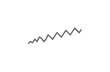
\begin{tikzpicture}[x=0.08em, y=0.08em, line width=0.4pt]
                \draw[FooterGray] (0,3) -- (1,4) -- (2,3.5) -- (3,5) -- (4,4) -- (5,6) -- (6,5.5) -- (7,4) -- (8,5) -- (9,7) -- (10,6) -- (11,5) -- (12,6.5) -- (13,8) -- (14,7) -- (15,6) -- (16,7.5) -- (17,9) -- (18,8) -- (19,7) -- (20,8.5) -- (21,10) -- (22,9) -- (23,8) -- (24,9.5);
            \end{tikzpicture}%
        }%
        \hskip0.5cm%
    }%
    \vskip6pt%
}

%=============================================================================
% PACHETE
%=============================================================================
\usepackage[utf8]{inputenc}
\usepackage[T1]{fontenc}
\usepackage{amsmath, amssymb, amsthm}
\usepackage{mathtools}
\usepackage{bm}
\usepackage{tikz}
\usetikzlibrary{arrows.meta, positioning, shapes, calc, decorations.pathreplacing, shadings}
\usepackage{booktabs}
\usepackage{multirow}
\usepackage{array}
\usepackage{graphicx}
\usepackage{hyperref}
\usepackage{colortbl}
\hypersetup{colorlinks=true, linkcolor=MainBlue, urlcolor=MainBlue}
\graphicspath{{../../logos/}{../../charts/}}
\hfuzz=2pt  % Suppress tiny overfull warnings (<2pt)
\vfuzz=2pt  % Suppress tiny vertical overfull warnings (<2pt)

%=============================================================================
% COMANDA QUANTLET
%=============================================================================
\newcommand{\quantlet}[2]{%
    \hfill\href{#2}{%
        \raisebox{-0.15em}{\includegraphics[height=0.7em]{ql_logo.png}}%
        \textcolor{MainBlue}{\tiny\ #1}%
    }%
}

%=============================================================================
% PAGINĂ TITLU PERSONALIZATĂ
%=============================================================================
\defbeamertemplate*{title page}{hybrid}[1][]
{
    \vspace{0.2cm}
    % Rând logo-uri - antet superior (cu linkuri clickabile)
    \begin{center}
        \href{https://www.ase.ro}{\includegraphics[height=1.0cm]{ase_logo.png}}\hspace{0.3cm}%
        \href{https://theida.net}{\includegraphics[height=1.0cm]{ida_logo.png}}\hspace{0.3cm}%
        \href{https://blockchain-research-center.com}{\includegraphics[height=1.0cm]{brc_logo.png}}\hspace{0.3cm}%
        \href{https://www.ai4efin.ase.ro}{\includegraphics[height=1.0cm]{ai4efin_logo.png}}\hspace{0.3cm}%
        \href{https://ipe.ro/new}{\includegraphics[height=1.0cm]{acad_logo.png}}\hspace{0.3cm}%
        \href{https://www.digital-finance-msca.com}{\includegraphics[height=1.0cm]{msca_logo.png}}%
    \end{center}

    \vspace{0.6cm}

    % Titlu principal cu logo-uri Q pe părți (cu linkuri clickabile)
    \begin{center}
        \begin{minipage}{0.1\textwidth}
            \centering
            \href{https://quantlet.com}{\includegraphics[height=1.1cm]{ql_logo.png}}
        \end{minipage}%
        \begin{minipage}{0.78\textwidth}
            \centering
            {\LARGE\bfseries\usebeamercolor[fg]{title}\inserttitle}

            \vspace{0.3cm}

            {\usebeamerfont{subtitle}\usebeamercolor[fg]{title}\insertsubtitle}
        \end{minipage}%
        \begin{minipage}{0.1\textwidth}
            \centering
            \href{https://quantinar.com}{\includegraphics[height=1.1cm]{qr_logo.png}}
        \end{minipage}
    \end{center}

    \vspace{0.6cm}

    % Autori (aliniere la stânga)
    \hspace{0.5cm}{\usebeamerfont{author}\insertauthor}

    \vspace{0.3cm}

    % Institut/Afilieri (aliniere la stânga)
    \hspace{0.5cm}\begin{minipage}[t]{0.9\textwidth}
        \raggedright\small\insertinstitute
    \end{minipage}
}

%=============================================================================
% MEDII PENTRU TEOREME
%=============================================================================
\theoremstyle{definition}
\setbeamertemplate{theorems}[numbered]
\newtheorem{defn}{Definiție}
\newtheorem{thm}{Teoremă}
\newtheorem{prop}{Propoziție}
\newtheorem{rmk}{Observație}

%=============================================================================
% COMENZI PERSONALIZATE
%=============================================================================
\newcommand{\E}{\mathbb{E}}
\newcommand{\Var}{\text{Var}}
\newcommand{\Cov}{\text{Cov}}
\newcommand{\Corr}{\text{Corr}}
\newcommand{\R}{\mathbb{R}}
\newcommand{\N}{\mathbb{N}}
\newcommand{\Z}{\mathbb{Z}}
\newcommand{\RMSE}{\text{RMSE}}
\newcommand{\MAE}{\text{MAE}}
\newcommand{\MAPE}{\text{MAPE}}

%=============================================================================
% INFORMAȚII TITLU
%=============================================================================
\title[Analiza Seriilor de Timp]{Analiza și Prognoza Seriilor de Timp}
\subtitle{Capitolul 2: Modele ARMA}
\author[D.T. Pele]{Daniel Traian PELE}
\institute{Academia de Studii Economice din București\\
IDA Institute Digital Assets\\
Blockchain Research Center\\
AI4EFin Artificial Intelligence for Energy Finance\\
Academia Română, Institutul de Prognoză Economică\\
MSCA Digital Finance}
\date{}

\begin{document}

% Pagina de titlu (fără antet/subsol)
{
\setbeamertemplate{headline}{}
\setbeamertemplate{footline}{}
\begin{frame}
    \titlepage
\end{frame}
}

%=============================================================================
% OBIECTIVE DE ÎNVĂȚARE
%=============================================================================
\begin{frame}{Obiective de Învățare}
    \begin{block}{La finalul acestui capitol, veți fi capabili să:}
    \begin{enumerate}\setlength{\itemsep}{0pt}
        \item[\textcolor{MainBlue}{\textbf{1.}}] \textbf{Definiți} și simulați procese AR($p$), MA($q$) și ARMA($p,q$)
        \item[\textcolor{MainBlue}{\textbf{2.}}] \textbf{Verificați} condițiile de staționaritate și invertibilitate
        \item[\textcolor{MainBlue}{\textbf{3.}}] \textbf{Identificați} ordinele $p$ și $q$ prin analiza ACF/PACF
        \item[\textcolor{MainBlue}{\textbf{4.}}] \textbf{Estimați} parametrii prin Yule-Walker, MLE și criterii informaționale (AIC, BIC)
        \item[\textcolor{MainBlue}{\textbf{5.}}] \textbf{Diagnosticați} modelul prin analiza reziduurilor și testul Ljung-Box
        \item[\textcolor{MainBlue}{\textbf{6.}}] \textbf{Prognozați} folosind modele ARMA cu intervale de încredere
        \item[\textcolor{MainBlue}{\textbf{7.}}] \textbf{Aplicați} metodologia Box-Jenkins pe date reale (pete solare)
    \end{enumerate}
    \end{block}
\end{frame}

%=============================================================================
% CUPRINS
%=============================================================================
\begin{frame}{Structura capitolului}
    \setbeamertemplate{section in toc}{\color{MainBlue}$\boxdot$~\inserttocsection}
    {\footnotesize
    \begin{columns}[T]
        \begin{column}{0.48\textwidth}
            \tableofcontents[sections={1-7}, hideallsubsections]
        \end{column}
        \begin{column}{0.48\textwidth}
            \tableofcontents[sections={8-13}, hideallsubsections]
        \end{column}
    \end{columns}
    }
\end{frame}

%=============================================================================
% MOTIVAȚIE
%=============================================================================
\section{Motivație}

\begin{frame}{De ce modele ARMA?}
    \vspace{-0.3cm}
    \begin{center}
        \includegraphics[width=0.92\textwidth, height=0.68\textheight, keepaspectratio]{ch2_motivation_stationary.pdf}
    \end{center}
    \vspace{-0.2cm}
    {\scriptsize
    \begin{itemize}
        \item \textbf{Procese AR}: Valoarea curentă depinde de valorile trecute $\succ$ comportament de revenire la medie
        \item \textbf{Procese MA}: Valoarea curentă depinde de șocurile trecute $\succ$ memorie scurtă
        \item \textbf{ARMA}: Combină ambele mecanisme pentru modelare flexibilă
    \end{itemize}
    }
    \quantlet{TSA\_ch2\_motivation}{https://github.com/QuantLet/TSA/tree/main/TSA_ch2/TSA_ch2_motivation}
\end{frame}

\begin{frame}{Identificarea modelului prin tipare ACF}
    \vspace{-0.3cm}
    \begin{center}
        \includegraphics[width=0.92\textwidth, height=0.68\textheight, keepaspectratio]{ch2_motivation_acf.pdf}
    \end{center}
    \vspace{-0.2cm}
    {\scriptsize
    \begin{exampleblock}{ACF reflectă structura modelului}
        \begin{itemize}\setlength{\itemsep}{0pt}
            \item \textbf{Tipare distincte}: AR: descreștere exponențială; MA: anulare bruscă; ARMA: descreștere mixtă
            \item \textbf{Identificare}: Analiza vizuală a ACF/PACF ghidează selecția ordinelor $p$ și $q$
        \end{itemize}
    \end{exampleblock}
    }
    \quantlet{TSA\_ch2\_motivation}{https://github.com/QuantLet/TSA/tree/main/TSA_ch2/TSA_ch2_motivation}
\end{frame}

%=============================================================================
% SECȚIUNEA 1: INTRODUCERE ȘI OPERATORUL LAG
%=============================================================================
\section{Introducere și operatorul lag}

\begin{frame}{Recapitulare: Staționaritatea}
    \vspace{-0.3cm}
    {\small
    \begin{block}{Din Capitolul 1}
        \begin{itemize}\setlength{\itemsep}{0pt}
            \item Un proces $\{X_t\}$ este \textbf{slab staționar} dacă:
            \begin{enumerate}\setlength{\itemsep}{0pt}
                \item $\E[X_t] = \mu$ (medie constantă)
                \item $\Var(X_t) = \sigma^2 < \infty$ (varianță constantă, finită)
                \item $\Cov(X_t, X_{t+h}) = \gamma(h)$ (covarianța depinde doar de lag-ul $h$)
            \end{enumerate}
        \end{itemize}
    \end{block}
    \vspace{-0.3cm}
    \begin{exampleblock}{De ce contează staționaritatea pentru ARMA}
        \begin{itemize}\setlength{\itemsep}{0pt}
            \item \textcolor{Forest}{Modelele ARMA presupun staționaritate} -- parametrii rămân stabili în timp, structura de autocorelație se menține
            \item \textcolor{Crimson}{Date nestaționare} $\succ$ diferențiați mai întâi (ARIMA, Cap. 3)
        \end{itemize}
    \end{exampleblock}
    \vspace{-0.3cm}
    \begin{alertblock}{Obiectivul capitolului}
        \begin{itemize}\setlength{\itemsep}{0pt}
            \item Modele parametrice pentru serii staționare $\succ$ combinând dependența de observațiile anterioare (AR) cu influența șocurilor aleatoare (MA)
        \end{itemize}
    \end{alertblock}
    }
\end{frame}

\begin{frame}{Operatorul lag (operatorul de întârziere)}
    \vspace{-0.2cm}
    \begin{defn}[Operatorul lag]
        \begin{itemize}\setlength{\itemsep}{0pt}
            \item \textbf{Operatorul lag} $L$ (sau operatorul de întârziere $B$) deplasează o serie de timp înapoi cu o perioadă: $L X_t = X_{t-1}$
        \end{itemize}
    \end{defn}
    \vspace{-0.2cm}
    \begin{block}{Proprietăți}
        \begin{itemize}\setlength{\itemsep}{0pt}
            \item $L^k X_t = X_{t-k}$ (deplasare înapoi cu $k$ perioade)
            \item $L^0 X_t = X_t$ (identitate)
            \item $(1-L)X_t = X_t - X_{t-1} = \Delta X_t$ (prima diferență)
            \item $(1-L)^d X_t = \Delta^d X_t$ (diferența de ordin $d$)
        \end{itemize}
    \end{block}
    \vspace{-0.2cm}
    \begin{exampleblock}{Polinoame lag}
        \begin{itemize}\setlength{\itemsep}{0pt}
            \item \textbf{Polinom AR}: $\phi(L) = 1 - \phi_1 L - \phi_2 L^2 - \cdots - \phi_p L^p$
            \item \textbf{Polinom MA}: $\theta(L) = 1 + \theta_1 L + \theta_2 L^2 + \cdots + \theta_q L^q$
        \end{itemize}
    \end{exampleblock}
    \quantlet{TSA\_ch2\_lag\_operator}{https://github.com/QuantLet/TSA/tree/main/TSA_ch2/TSA_ch2_lag_operator}
\end{frame}

\begin{frame}{Operatorul lag: ilustrație vizuală}
    \begin{center}
        \includegraphics[width=0.88\textwidth, height=0.68\textheight, keepaspectratio]{lag_operator.pdf}
    \end{center}
    \vspace{-0.2cm}
    {\scriptsize
    \begin{block}{Rolul operatorului lag}
        \begin{itemize}\setlength{\itemsep}{0pt}
            \item \textbf{Fundamentul notației}: Permite scrierea compactă a ecuațiilor cu diferențe
            \item \textbf{Utilitate}: Facilitează manipularea algebrică a modelelor ARMA
        \end{itemize}
    \end{block}
    }
    \quantlet{TSA\_ch2\_lag\_operator}{https://github.com/QuantLet/TSA/tree/main/TSA_ch2/TSA_ch2_lag_operator}
\end{frame}

\begin{frame}{Procesul de zgomot alb}
    \vspace{-0.2cm}
    \begin{defn}[Zgomot Alb]
        \begin{itemize}\setlength{\itemsep}{0pt}
            \item Un proces $\{\varepsilon_t\}$ este \textbf{zgomot alb}, notat $\varepsilon_t \sim WN(0, \sigma^2)$, dacă:
            \begin{enumerate}
                \item $\E[\varepsilon_t] = 0$ pentru toți $t$
                \item $\Var(\varepsilon_t) = \sigma^2$ pentru toți $t$
                \item $\Cov(\varepsilon_t, \varepsilon_s) = 0$ pentru toți $t \neq s$
            \end{enumerate}
        \end{itemize}
    \end{defn}
    \vspace{-0.2cm}
    {\footnotesize
    \begin{block}{Proprietăți}
        \begin{itemize}\setlength{\itemsep}{0pt}
            \item \textbf{Element de bază}: Zgomotul alb stă la baza tuturor modelelor ARMA
            \item \textbf{ACF}: $\rho(0) = 1$, $\rho(h) = 0$ pentru $h \neq 0$; PACF: același tipar
            \item \textbf{Zgomot alb Gaussian}: $\varepsilon_t \sim N(0, \sigma^2)$ i.i.d.
            \item \textbf{Nepredictibil}: Zgomotul alb \textit{nu} este predictibil $\succ$ este pur aleatoriu
        \end{itemize}
    \end{block}
    }
\end{frame}

\begin{frame}{Zgomot alb: ilustrare vizuală}
    \vspace{-0.3cm}
    \begin{center}
        \includegraphics[width=0.92\textwidth, height=0.55\textheight, keepaspectratio]{ch2_white_noise.pdf}
    \end{center}
    \vspace{-0.3cm}
    {\scriptsize
    \begin{block}{Caracteristici cheie}
        \begin{itemize}\setlength{\itemsep}{0pt}
            \item \textbf{Stânga}: Fluctuații aleatorii, fără tipare, varianță constantă
            \item \textbf{Dreapta}: ACF doar un vârf la lag 0; celelalte în limitele de semnificație $\succ$ fără dependență liniară
        \end{itemize}
    \end{block}
    }
    \quantlet{TSA\_ch2\_white\_noise}{https://github.com/QuantLet/TSA/tree/main/TSA_ch2/TSA_ch2_white_noise}
\end{frame}

%=============================================================================
% SECȚIUNEA 2: MODELE AR
%=============================================================================
\section{Modele autoregresive (AR)}

\begin{frame}{Modelul AR(1): definiție}
    \vspace{-0.2cm}
    \begin{defn}[Proces AR(1)]
        \begin{itemize}\setlength{\itemsep}{0pt}
            \item Un \textbf{proces autoregresiv de ordin 1} este: $X_t = c + \phi X_{t-1} + \varepsilon_t$
            \item $\varepsilon_t \sim WN(0, \sigma^2)$ și $|\phi| < 1$ pentru staționaritate
        \end{itemize}
    \end{defn}
    \vspace{-0.2cm}
    \begin{columns}[T]
        \begin{column}{0.48\textwidth}
        \begin{block}{Interpretare}
            \begin{itemize}\setlength{\itemsep}{0pt}
                \item $c$: constantă (interceptul)
                \item $\phi$: coeficient autoregresiv
                \begin{itemize}
                    \item Măsoară persistența seriei
                \end{itemize}
                \item $\varepsilon_t$: inovație (șoc)
            \end{itemize}
        \end{block}
        \end{column}
        \begin{column}{0.48\textwidth}
        \begin{exampleblock}{Notație cu operatorul lag}
            \begin{itemize}\setlength{\itemsep}{0pt}
                \item $(1 - \phi L)X_t = c + \varepsilon_t$
                \item $\phi(L) X_t = c + \varepsilon_t$
                \item $\phi(L) = 1 - \phi L$
            \end{itemize}
        \end{exampleblock}
        \end{column}
    \end{columns}
\end{frame}

\begin{frame}{AR(1): ilustrație vizuală}
    \vspace{-0.3cm}
    \begin{center}
        \includegraphics[width=0.95\textwidth, height=0.60\textheight, keepaspectratio]{ch2_def_ar1.pdf}
    \end{center}
    \vspace{-0.3cm}
    {\scriptsize
    \begin{block}{Interpretarea vizuală}
        \begin{itemize}\setlength{\itemsep}{0pt}
            \item \textbf{$\phi$ pozitiv}: Fluctuații persistente, revenire graduală la medie
            \item \textbf{$\phi$ negativ}: Comportament oscilant, alternând în jurul mediei
            \item $|\phi|$ mai mare $\succ$ persistență mai mare, revenire mai lentă
        \end{itemize}
    \end{block}
    }
    \quantlet{TSA\_ch2\_ar1}{https://github.com/QuantLet/TSA/tree/main/TSA_ch2/TSA_ch2_ar1}
\end{frame}

\begin{frame}{Condiția de staționaritate AR(1)}
    \vspace{-0.2cm}
    \begin{alertblock}{Condiție necesară și suficientă: $|\phi| < 1$}
        \begin{itemize}\setlength{\itemsep}{0pt}
            \item Rădăcina ecuației caracteristice trebuie să fie în afara cercului unitate
        \end{itemize}
    \end{alertblock}
    \vspace{-0.2cm}
    \begin{columns}[T]
        \begin{column}{0.48\textwidth}
        \begin{exampleblock}{\textcolor{Forest}{Staționar ($|\phi| < 1$)}}
            \begin{itemize}\setlength{\itemsep}{0pt}
                \item Șocurile se diminuează în timp
                \begin{itemize}
                    \item Procesul revine la medie
                    \item Varianță finită, stabilă
                \end{itemize}
            \end{itemize}
        \end{exampleblock}
        \end{column}
        \begin{column}{0.48\textwidth}
        \begin{alertblock}{\textcolor{white}{Nestaționar ($|\phi| \geq 1$)}}
            \begin{itemize}\setlength{\itemsep}{0pt}
                \item $|\phi| = 1$: mers aleatoriu
                \begin{itemize}
                    \item Rădăcină unitate, varianță $\to \infty$
                \end{itemize}
                \item $|\phi| > 1$: proces exploziv
            \end{itemize}
        \end{alertblock}
        \end{column}
    \end{columns}
    \vspace{-0.2cm}
    \begin{block}{Ecuația caracteristică}
        \begin{itemize}\setlength{\itemsep}{0pt}
            \item $\phi(z) = 1 - \phi z = 0 \implies z = 1/\phi$
            \item Staționaritate $\Leftrightarrow$ rădăcina în afara cercului unitate ($|z|>1$)
        \end{itemize}
    \end{block}
\end{frame}

\begin{frame}{Proprietățile AR(1)}
    \vspace{-0.2cm}
    \begin{block}{AR(1) staționar cu $|\phi| < 1$}
    \begin{itemize}\setlength{\itemsep}{0pt}
    \item Proprietățile momentelor:
    \end{itemize}
    \vspace{-0.2cm}
    \begin{columns}[T]
        \begin{column}{0.48\textwidth}
        {\small \textbf{Media:} $\mu = \E[X_t] = \frac{c}{1-\phi}$}

        {\small \textbf{Varianța:} $\gamma(0) = \Var(X_t) = \frac{\sigma^2}{1-\phi^2}$}
        \end{column}
        \begin{column}{0.48\textwidth}
        {\small \textbf{Autocovarianța:} $\gamma(h) = \frac{\phi^h \sigma^2}{1-\phi^2}$}

        {\small \textbf{Autocorelația (ACF):} $\rho(h) = \phi^h$}
        \end{column}
    \end{columns}
    \end{block}
    \vspace{-0.2cm}
    \begin{alertblock}{Observație cheie}
        \begin{itemize}\setlength{\itemsep}{0pt}
            \item \textbf{Semnătura AR(1)}: ACF scade exponențial cu factorul $\phi$
            \begin{itemize}
                \item $\phi > 0$: descreștere monotonă spre zero
                \item $\phi < 0$: oscilații amortizate (semne alternante)
            \end{itemize}
        \end{itemize}
    \end{alertblock}
    \quantlet{TSA\_ch2\_ar1}{https://github.com/QuantLet/TSA/tree/main/TSA_ch2/TSA_ch2_ar1}
\end{frame}

\begin{frame}{Demonstrație: media AR(1)}
    \vspace{-0.3cm}
    \begin{block}{Afirmație}
        \begin{itemize}\setlength{\itemsep}{0pt}
            \item Pentru AR(1): $X_t = c + \phi X_{t-1} + \varepsilon_t$, media este $\mu = \frac{c}{1-\phi}$
        \end{itemize}
    \end{block}
    \vspace{-0.3cm}
    {\small
    \begin{exampleblock}{Demonstrație}
        \begin{itemize}\setlength{\itemsep}{0pt}
            \item Luăm speranța ambelor părți: $\E[X_t] = c + \phi \E[X_{t-1}] + \E[\varepsilon_t]$
            \item Prin staționaritate, $\E[X_t] = \E[X_{t-1}] = \mu$, și $\E[\varepsilon_t] = 0$: $\mu = c + \phi \mu$
            \item Rezolvând: $\mu - \phi\mu = c \implies \mu(1-\phi) = c \implies \boxed{\mu = \frac{c}{1-\phi}}$
        \end{itemize}
    \end{exampleblock}
    }
    \vspace{-0.2cm}
    \begin{alertblock}{Cerință}
        \begin{itemize}\setlength{\itemsep}{0pt}
            \item \textbf{Condiție necesară}: $\phi \neq 1$ pentru ca media să fie definită
            \begin{itemize}
                \item Dacă $\phi = 1$ (rădăcină unitară), media este nedefinită
                \item Procesul devine mers aleatoriu (nestaționaritate)
            \end{itemize}
        \end{itemize}
    \end{alertblock}
\end{frame}

\begin{frame}{Demonstrație: varianța AR(1)}
    \vspace{-0.3cm}
    \begin{block}{Afirmație}
        \begin{itemize}\setlength{\itemsep}{0pt}
            \item $\Var(X_t) = \frac{\sigma^2}{1-\phi^2}$
        \end{itemize}
    \end{block}
    \vspace{-0.3cm}
    {\small
    \begin{exampleblock}{Demonstrație}
        \begin{itemize}\setlength{\itemsep}{0pt}
            \item Presupunem $c=0$. Luăm varianța din $X_t = \phi X_{t-1} + \varepsilon_t$:
            \item $\Var(X_t) = \phi^2 \Var(X_{t-1}) + \Var(\varepsilon_t) + 2\phi\underbrace{\Cov(X_{t-1}, \varepsilon_t)}_{=0}$
            \item Prin staționaritate, $\Var(X_t) = \Var(X_{t-1}) = \gamma(0)$:
            \item $\gamma(0) = \phi^2 \gamma(0) + \sigma^2 \implies \gamma(0)(1-\phi^2) = \sigma^2 \implies \boxed{\gamma(0) = \frac{\sigma^2}{1-\phi^2}}$
        \end{itemize}
    \end{exampleblock}
    }
    \vspace{-0.2cm}
    \begin{alertblock}{Notă}
        \begin{itemize}\setlength{\itemsep}{0pt}
            \item Necesită $|\phi| < 1$ pentru varianță pozitivă. Când $|\phi| \to 1$, varianța $\to \infty$
        \end{itemize}
    \end{alertblock}
\end{frame}

\begin{frame}{Demonstrație: funcția de autocorelație AR(1)}
    \vspace{-0.3cm}
    \begin{block}{Afirmație: $\rho(h) = \phi^h$ pentru $h \geq 0$}
        \begin{itemize}\setlength{\itemsep}{0pt}
            \item Găsim autocovarianța $\gamma(h) = \Cov(X_t, X_{t-h})$
        \end{itemize}
    \end{block}
    \vspace{-0.3cm}
    {\small
    \begin{exampleblock}{Demonstrație}
        \begin{itemize}\setlength{\itemsep}{0pt}
            \item Înmulțim $X_t = \phi X_{t-1} + \varepsilon_t$ cu $X_{t-h}$ și luăm media:
            \item $\E[X_t X_{t-h}] = \phi \E[X_{t-1} X_{t-h}] + \E[\varepsilon_t X_{t-h}]$
            \item Pentru $h \geq 1$: $\E[\varepsilon_t X_{t-h}] = 0$ $\succ$ $\gamma(h) = \phi \gamma(h-1)$
            \item Relație recursivă de la $\gamma(0)$: $\gamma(1) = \phi\gamma(0)$, $\gamma(2) = \phi^2\gamma(0)$, $\ldots$ $\boxed{\gamma(h) = \phi^h\gamma(0)}$
            \item ACF: $\rho(h) = \frac{\gamma(h)}{\gamma(0)} = \frac{\phi^h\gamma(0)}{\gamma(0)} = \boxed{\phi^h}$
        \end{itemize}
    \end{exampleblock}
    }
\end{frame}

\begin{frame}{Varianța AR(1) ca funcție de $\phi$}
    \vspace{-0.2cm}
    \begin{center}
        \includegraphics[width=0.85\textwidth, height=0.55\textheight, keepaspectratio]{ar1_variance.pdf}
    \end{center}
    \vspace{-0.3cm}
    {\scriptsize
    \begin{block}{Observații}
        \begin{itemize}\setlength{\itemsep}{0pt}
            \item Pe măsură ce $|\phi| \to 1$, varianța explodează $\succ$ nestaționaritate
            \item Pentru $\phi = 0$: $\gamma(0) = \sigma^2$ (zgomot alb); varianța crește monoton cu $|\phi|$
        \end{itemize}
    \end{block}
    }
    \quantlet{TSA\_ch2\_ar1}{https://github.com/QuantLet/TSA/tree/main/TSA_ch2/TSA_ch2_ar1}
\end{frame}

\begin{frame}{Simulări AR(1): efectul lui $\phi$}
    \vspace{-0.3cm}
    \begin{center}
        \includegraphics[width=0.82\textwidth, height=0.60\textheight, keepaspectratio]{ch2_ar1_simulations.pdf}
    \end{center}
    \vspace{-0.2cm}
    {\scriptsize
    \begin{block}{Interpretare}
        \begin{itemize}\setlength{\itemsep}{0pt}
            \item Valori diferite ale lui $\phi$ produc comportamente distincte: $|\phi|$ mai mare $\succ$ mai multă persistență
            \item $\phi$ pozitiv creează evoluții netede; $\phi$ negativ creează oscilații
            \item Pe măsură ce $|\phi| \to 1$, procesul se apropie de nestaționaritate
        \end{itemize}
    \end{block}
    }
    \quantlet{TSA\_ch2\_ar1\_simulation}{https://github.com/QuantLet/TSA/tree/main/TSA_ch2/TSA_ch2_ar1_simulation}
\end{frame}

\begin{frame}{ACF teoretic AR(1)}
    \vspace{-0.2cm}
    \begin{center}
        \includegraphics[width=0.85\textwidth, height=0.63\textheight, keepaspectratio]{ar1_theoretical_acf.pdf}
    \end{center}
    \vspace{-0.2cm}
    {\scriptsize
    \begin{block}{Tipar ACF}
        \begin{itemize}\setlength{\itemsep}{0pt}
            \item \textbf{Formula}: $\rho(h) = \phi^h$ $\succ$ descreștere exponențială
            \item $\phi > 0$: descreștere monotonă; $\phi < 0$: semne alternante
        \end{itemize}
    \end{block}
    }
    \quantlet{TSA\_ch2\_ar1}{https://github.com/QuantLet/TSA/tree/main/TSA_ch2/TSA_ch2_ar1}
\end{frame}

\begin{frame}{Demonstrație: condiția de staționaritate AR(1)}
    \vspace{-0.3cm}
    \begin{block}{Afirmație}
        \begin{itemize}\setlength{\itemsep}{0pt}
            \item AR(1) este staționar dacă și numai dacă $|\phi| < 1$
        \end{itemize}
    \end{block}
    \vspace{-0.3cm}
    {\small
    \begin{exampleblock}{Demonstrație}
        \begin{itemize}\setlength{\itemsep}{0pt}
            \item Substituție recursivă: $X_t = \phi X_{t-1} + \varepsilon_t = \phi(\phi X_{t-2} + \varepsilon_{t-1}) + \varepsilon_t = \cdots$
            \item După $n$ pași: $X_t = \phi^n X_{t-n} + \sum_{j=0}^{n-1}\phi^j\varepsilon_{t-j}$
            \item Dacă $|\phi| < 1$: $\phi^n \to 0$ când $n \to \infty$, deci $X_t = \sum_{j=0}^{\infty}\phi^j\varepsilon_{t-j}$
            \item Varianță finită: $\Var(X_t) = \sigma^2\sum_{j=0}^{\infty}\phi^{2j} = \frac{\sigma^2}{1-\phi^2} < \infty$ \quad (serie geometrică)
        \end{itemize}
    \end{exampleblock}
    }
    \vspace{-0.2cm}
    \begin{alertblock}{Concluzie}
        \begin{itemize}\setlength{\itemsep}{0pt}
            \item Converge $\iff |\phi| < 1$. Pentru $|\phi| \geq 1$, termenul $\phi^n X_{t-n}$ nu dispare $\Rightarrow$ varianță infinită
        \end{itemize}
    \end{alertblock}
\end{frame}

\begin{frame}{ACF și PACF AR(1): teorie vs eșantion}
    \vspace{-0.3cm}
    \begin{center}
        \includegraphics[width=0.82\textwidth, height=0.60\textheight, keepaspectratio]{ch2_ar1_acf_pacf.pdf}
    \end{center}
    \vspace{-0.2cm}
    {\scriptsize
    \begin{block}{Interpretare}
        \begin{itemize}\setlength{\itemsep}{0pt}
            \item \textbf{ACF}: Descreștere exponențială cu factorul $\phi$; formula: $\rho(h) = \phi^h$
            \item \textbf{PACF}: Un singur vârf la lag 1, apoi se anulează $\succ$ identifică AR(1)
            \item Estimările din eșantion fluctuează în jurul valorilor teoretice
        \end{itemize}
    \end{block}
    }
    \quantlet{TSA\_ch2\_ar1}{https://github.com/QuantLet/TSA/tree/main/TSA_ch2/TSA_ch2_ar1}
\end{frame}

\begin{frame}{Funcția de autocorelație parțială (PACF)}
    \vspace{-0.3cm}
    \begin{defn}[PACF]
        \begin{itemize}\setlength{\itemsep}{0pt}
            \item \textbf{Autocorelația parțială} de ordin $k$, notată $\pi_k$, măsoară corelația dintre $X_t$ și $X_{t-k}$ \textbf{după eliminarea} efectelor liniare ale variabilelor intermediare $X_{t-1}, \ldots, X_{t-k+1}$
        \end{itemize}
    \end{defn}
    \vspace{-0.3cm}
    {\small
    \begin{columns}[T]
        \begin{column}{0.48\textwidth}
        \begin{block}{Definiție formală}
            \begin{itemize}\setlength{\itemsep}{0pt}
                \item $\pi_1 = \rho(1)$
                \item Pentru $k \geq 2$: $\pi_k$ este ultimul coeficient din: $X_t = \alpha_1 X_{t-1} + \cdots + \alpha_k X_{t-k} + e_t$
                \item $\pi_k = \alpha_k$ (coeficientul lui $X_{t-k}$)
            \end{itemize}
        \end{block}
        \end{column}
        \begin{column}{0.48\textwidth}
        \begin{exampleblock}{Calculul prin Yule-Walker}
            \begin{itemize}\setlength{\itemsep}{0pt}
                \item Se rezolvă ecuațiile Yule-Walker de ordin $k$
                \item $\pi_k$ = ultimul element al vectorului soluție
            \end{itemize}
        \end{exampleblock}
        \vspace{-0.2cm}
        \begin{alertblock}{Utilitate}
            \begin{itemize}\setlength{\itemsep}{0pt}
                \item \textbf{Identificare}: PACF determină ordinul $p$ al unui model AR
                \begin{itemize}
                    \item PACF se anulează după lag $p$
                \end{itemize}
            \end{itemize}
        \end{alertblock}
        \end{column}
    \end{columns}
    }
\end{frame}

\begin{frame}{Tipare ACF și PACF AR(1)}
    \begin{columns}[T]
        \begin{column}{0.48\textwidth}
        \begin{block}{ACF al AR(1)}
            \begin{itemize}\setlength{\itemsep}{0pt}
                \item Scade exponențial: $\rho(h) = \phi^h$
                \begin{itemize}
                    \item $\phi > 0$: toate pozitive
                    \item $\phi < 0$: semne alternante
                \end{itemize}
            \end{itemize}
        \end{block}
        \end{column}
        \begin{column}{0.48\textwidth}
        \begin{block}{PACF al AR(1)}
            \begin{itemize}\setlength{\itemsep}{0pt}
                \item \textbf{Se anulează după lag 1}
                \begin{itemize}
                    \item $\pi_1 = \phi$, $\pi_k = 0$ pentru $k > 1$
                \end{itemize}
            \end{itemize}
        \end{block}
        \end{column}
    \end{columns}

    \vspace{0.1cm}
    \begin{center}
    \begin{tabular}{lcc}
        \toprule
        & \textbf{ACF} & \textbf{PACF} \\
        \midrule
        AR(1) & Descreștere exponențială & Se anulează la lag 1 \\
        \bottomrule
    \end{tabular}
    \end{center}

    \vspace{0.1cm}
    \begin{alertblock}{Tipar cheie}
        \begin{itemize}\setlength{\itemsep}{0pt}
            \item Acesta este tiparul cheie de identificare pentru AR(1)!
        \end{itemize}
    \end{alertblock}
\end{frame}

\begin{frame}{Modelul AR(p): forma generală}
    \vspace{-0.2cm}
    \begin{defn}[Proces AR(p)]
        \begin{itemize}\setlength{\itemsep}{0pt}
            \item Un \textbf{proces autoregresiv de ordin p} este: $X_t = c + \phi_1 X_{t-1} + \phi_2 X_{t-2} + \cdots + \phi_p X_{t-p} + \varepsilon_t$
            \item \textbf{Operator lag}: $\phi(L) X_t = c + \varepsilon_t$, unde $\phi(L) = 1 - \phi_1 L - \phi_2 L^2 - \cdots - \phi_p L^p$
        \end{itemize}
    \end{defn}
    \vspace{-0.2cm}
    \begin{block}{Condiție de staționaritate}
        \begin{itemize}\setlength{\itemsep}{0pt}
            \item Toate rădăcinile lui $\phi(z) = 0$ trebuie să se afle \textbf{în afara} cercului unitate
            \item Echivalent: toate rădăcinile au modul $> 1$
        \end{itemize}
    \end{block}
    \vspace{-0.2cm}
    \begin{exampleblock}{Tiparul PACF}
        \begin{itemize}\setlength{\itemsep}{0pt}
            \item PACF se anulează după lag $p$
            \item ACF scade (exponențial sau cu oscilații amortizate)
        \end{itemize}
    \end{exampleblock}
\end{frame}

\begin{frame}{AR(p): ilustrație vizuală}
    \vspace{-0.2cm}
    \begin{center}
        \includegraphics[width=0.92\textwidth, height=0.60\textheight, keepaspectratio]{ch2_def_arp.pdf}
    \end{center}
    \vspace{-0.3cm}
    {\scriptsize
    \begin{block}{Observații}
        \begin{itemize}\setlength{\itemsep}{0pt}
            \item AR(2) poate prezenta comportament pseudo-ciclic (rădăcini complexe); ACF sinusoidală amortizată
            \item PACF se anulează după lag 2 $\succ$ tiparul cheie de identificare
        \end{itemize}
    \end{block}
    }
    \quantlet{TSA\_ch2\_ar2}{https://github.com/QuantLet/TSA/tree/main/TSA_ch2/TSA_ch2_ar2}
\end{frame}

\begin{frame}{Staționaritatea AR(2): vizualizarea cercului unitate}
    \vspace{-0.3cm}
    \begin{center}
        \includegraphics[width=0.85\textwidth, height=0.58\textheight, keepaspectratio]{unit_circle_stationarity.pdf}
    \end{center}
    \vspace{-0.3cm}
    {\scriptsize
    \begin{block}{Polinomul caracteristic și condiția cercului unitate}
        \begin{itemize}\setlength{\itemsep}{0pt}
            \item \textbf{Polinomul caracteristic} al unui proces AR($p$): $\phi(z) = 1 - \phi_1 z - \phi_2 z^2 - \cdots - \phi_p z^p$
            \item Toate rădăcinile lui $\phi(z) = 0$ trebuie să se afle \textbf{în afara} cercului unitate ($|z| > 1$)
            \item Rădăcini pe cerc: nestaționar; rădăcini în interior: proces exploziv
        \end{itemize}
    \end{block}
    }
    \quantlet{TSA\_ch2\_stationarity}{https://github.com/QuantLet/TSA/tree/main/TSA_ch2/TSA_ch2_stationarity}
\end{frame}

\begin{frame}{Triunghiul de staționaritate AR(2)}
    \vspace{-0.3cm}
    \begin{center}
        \includegraphics[width=0.82\textwidth, height=0.52\textheight, keepaspectratio]{ch2_ar2_stationarity.pdf}
    \end{center}
    \vspace{-0.3cm}
    {\scriptsize
    \begin{block}{Regiunea de staționaritate}
        \begin{itemize}\setlength{\itemsep}{0pt}
            \item Regiunea triunghiulară definește combinațiile de parametri AR(2) staționari
            \item \textbf{Granițe}: $\phi_1 + \phi_2 < 1$, $\phi_2 - \phi_1 < 1$ și $|\phi_2| < 1$
            \item Punctele din afara regiunii $\succ$ procese nestaționare sau explozive
        \end{itemize}
    \end{block}
    }
    \quantlet{TSA\_ch2\_stationarity}{https://github.com/QuantLet/TSA/tree/main/TSA_ch2/TSA_ch2_stationarity}
\end{frame}

\begin{frame}{Rădăcinile polinomului caracteristic}
    \vspace{-0.3cm}
    \begin{center}
        \includegraphics[width=0.88\textwidth, height=0.60\textheight, keepaspectratio]{characteristic_roots.pdf}
    \end{center}
    \vspace{-0.3cm}
    {\scriptsize
    \begin{block}{Tipuri de rădăcini}
        \begin{itemize}\setlength{\itemsep}{0pt}
            \item \textbf{Rădăcini reale}: descreștere exponențială în ACF
            \item \textbf{Rădăcini complexe}: oscilații amortizate (pseudo-cicluri)
            \item Toate rădăcinile trebuie să fie în afara cercului unitate
        \end{itemize}
    \end{block}
    }
    \quantlet{TSA\_ch2\_stationarity}{https://github.com/QuantLet/TSA/tree/main/TSA_ch2/TSA_ch2_stationarity}
\end{frame}

\begin{frame}{Modelul AR(2)}
    \vspace{-0.2cm}
    \begin{defn}[Proces AR(2)]
        \begin{itemize}\setlength{\itemsep}{0pt}
            \item $X_t = c + \phi_1 X_{t-1} + \phi_2 X_{t-2} + \varepsilon_t$
        \end{itemize}
    \end{defn}
    \vspace{-0.2cm}
    \begin{block}{Condiții de staționaritate}
        \begin{itemize}\setlength{\itemsep}{0pt}
            \item $\phi_1 + \phi_2 < 1$; \quad $\phi_2 - \phi_1 < 1$; \quad $|\phi_2| < 1$
        \end{itemize}
    \end{block}
    \vspace{-0.2cm}
    \begin{exampleblock}{Comportamentul ACF}
        \begin{itemize}\setlength{\itemsep}{0pt}
            \item \textbf{Rădăcini reale}: amestec de două descreșteri exponențiale
            \item \textbf{Rădăcini complexe}: tipar sinusoidal amortizat (pseudo-cicluri)
            \item \textbf{PACF}: Se anulează după lag 2 ($\pi_k = 0$ pentru $k > 2$)
        \end{itemize}
    \end{exampleblock}
    \quantlet{TSA\_ch2\_ar2}{https://github.com/QuantLet/TSA/tree/main/TSA_ch2/TSA_ch2_ar2}
\end{frame}

%=============================================================================
% SECȚIUNEA 3: MODELE MA
%=============================================================================
\section{Modele de medie mobilă (MA)}

\begin{frame}{Modelul MA(1): definiție}
    \vspace{-0.2cm}
    \begin{defn}[Proces MA(1)]
        \begin{itemize}\setlength{\itemsep}{0pt}
            \item Un \textbf{proces de medie mobilă de ordin 1} este: $X_t = \mu + \varepsilon_t + \theta \varepsilon_{t-1}$
            \item $\varepsilon_t \sim WN(0, \sigma^2)$
        \end{itemize}
    \end{defn}
    \vspace{-0.2cm}
    \begin{columns}[T]
        \begin{column}{0.48\textwidth}
        \begin{block}{Interpretare}
            \begin{itemize}\setlength{\itemsep}{0pt}
                \item $\mu$: media procesului
                \item $\theta$: coeficient MA
                \begin{itemize}
                    \item Măsoară impactul șocului trecut
                \end{itemize}
                \item Depinde de $\varepsilon_t$ și $\varepsilon_{t-1}$
            \end{itemize}
        \end{block}
        \end{column}
        \begin{column}{0.48\textwidth}
        \begin{exampleblock}{Notație cu operatorul lag}
            \begin{itemize}\setlength{\itemsep}{0pt}
                \item $X_t = \mu + \theta(L)\varepsilon_t$
                \item $\theta(L) = 1 + \theta L$
            \end{itemize}
        \end{exampleblock}
        \vspace{-0.2cm}
        \begin{alertblock}{Proprietate cheie}
            \begin{itemize}\setlength{\itemsep}{0pt}
                \item \textbf{Staționaritate garantată}: Procesele MA sunt întotdeauna staționare
                \begin{itemize}
                    \item Nu depinde de valoarea lui $\theta$
                \end{itemize}
            \end{itemize}
        \end{alertblock}
        \end{column}
    \end{columns}
\end{frame}

\begin{frame}{MA(1): ilustrație vizuală}
    \vspace{-0.2cm}
    \begin{center}
        \includegraphics[width=0.92\textwidth, height=0.55\textheight, keepaspectratio]{ch2_def_ma1.pdf}
    \end{center}
    \vspace{-0.3cm}
    {\scriptsize
    \begin{block}{Interpretare vizuală}
        \begin{itemize}\setlength{\itemsep}{0pt}
            \item \textbf{Panoul stâng}: Serie MA(1) $\succ$ revenire rapidă la medie
            \item \textbf{Panoul drept}: ACF cu \textbf{anulare după lag 1}; PACF descreștere exponențială
        \end{itemize}
    \end{block}
    }
    \quantlet{TSA\_ch2\_ma1}{https://github.com/QuantLet/TSA/tree/main/TSA_ch2/TSA_ch2_ma1}
\end{frame}

\begin{frame}{Proprietățile MA(1)}
    \vspace{-0.3cm}
    {\small
    \begin{block}{MA(1): $X_t = \mu + \varepsilon_t + \theta \varepsilon_{t-1}$}
        \begin{itemize}\setlength{\itemsep}{0pt}
            \item \textbf{Media}: $\E[X_t] = \mu$; \quad \textbf{Varianța}: $\gamma(0) = \sigma^2(1 + \theta^2)$
            \item \textbf{Autocovarianța}: $\gamma(1) = \theta\sigma^2$, $\gamma(h) = 0$ $(h > 1)$
            \item \textbf{ACF}: $\rho(1) = \frac{\theta}{1+\theta^2}$, $\rho(h) = 0$ $(h > 1)$
        \end{itemize}
    \end{block}
    \vspace{-0.3cm}
    \begin{alertblock}{Observație cheie}
        \begin{itemize}\setlength{\itemsep}{0pt}
            \item \textbf{Semnătura MA(1)}: ACF se anulează după lag 1
            \begin{itemize}
                \item $\rho(1) \neq 0$, dar $\rho(h) = 0$ pentru $h > 1$; tipar opus față de AR(1)
            \end{itemize}
        \end{itemize}
    \end{alertblock}
    }
    \quantlet{TSA\_ch2\_ma1}{https://github.com/QuantLet/TSA/tree/main/TSA_ch2/TSA_ch2_ma1}
\end{frame}

\begin{frame}{Demonstrație: varianța și autocovarianța MA(1)}
    \vspace{-0.3cm}
    {\small
    \begin{block}{Punct de plecare: $X_t = \varepsilon_t + \theta\varepsilon_{t-1}$ (presupunând $\mu = 0$)}
        \begin{itemize}\setlength{\itemsep}{0pt}
            \item \textbf{Varianța}:
        \end{itemize}
        \vspace{-0.3cm}
        \begin{align*}
        \gamma(0) &= \Var(\varepsilon_t + \theta\varepsilon_{t-1}) = \sigma^2 + \theta^2\sigma^2 + 0 = \boxed{\sigma^2(1+\theta^2)}
        \end{align*}
    \end{block}
    \vspace{-0.4cm}
    \begin{exampleblock}{Autocovarianța la lag 1}
        \begin{itemize}\setlength{\itemsep}{0pt}
            \item $\gamma(1) = \Cov(\varepsilon_t + \theta\varepsilon_{t-1}, \varepsilon_{t-1} + \theta\varepsilon_{t-2})$
            \item $= \Cov(\varepsilon_t, \varepsilon_{t-1}) + \theta\Cov(\varepsilon_t, \varepsilon_{t-2}) + \theta\Cov(\varepsilon_{t-1}, \varepsilon_{t-1}) + \theta^2\Cov(\varepsilon_{t-1}, \varepsilon_{t-2})$
            \item $= 0 + 0 + \theta\sigma^2 + 0 = \boxed{\theta\sigma^2}$
        \end{itemize}
    \end{exampleblock}
    \vspace{-0.3cm}
    \begin{alertblock}{Autocovarianța la lag $h \geq 2$}
        \begin{itemize}\setlength{\itemsep}{0pt}
            \item Niciun termen $\varepsilon$ comun $\succ$ $\gamma(h) = 0$
        \end{itemize}
    \end{alertblock}
    }
\end{frame}

\begin{frame}{Demonstrație: maximul ACF pentru MA(1)}
    \vspace{-0.3cm}
    {\small
    \begin{block}{Afirmație: $|\rho(1)| \leq 0.5$ pentru orice valoare a lui $\theta$}
        \begin{itemize}\setlength{\itemsep}{0pt}
            \item ACF la lag 1: $\rho(1) = \frac{\theta}{1+\theta^2}$
            \item Derivăm: $\frac{d\rho(1)}{d\theta} = \frac{1-\theta^2}{(1+\theta^2)^2} = 0$ $\succ$ $\theta = \pm 1$
            \item La aceste valori: $\rho(1)\big|_{\theta=1} = \frac{1}{2}$, $\rho(1)\big|_{\theta=-1} = -\frac{1}{2}$
        \end{itemize}
    \end{block}
    }
    \begin{exampleblock}{Implicație}
        \begin{itemize}\setlength{\itemsep}{0pt}
            \item \textbf{Test practic}: Dacă $|\hat{\rho}(1)| > 0.5$ din date, procesul \textbf{nu} este MA(1)
            \begin{itemize}
                \item Maximul $|\rho(1)| = 0.5$ se atinge la $\theta = \pm 1$
                \item Considerați modele AR sau ARMA ca alternative
            \end{itemize}
        \end{itemize}
    \end{exampleblock}
\end{frame}

\begin{frame}{Demonstrație: ACF pentru MA(1)}
    \vspace{-0.3cm}
    \begin{block}{Afirmație: $\rho(1) = \frac{\theta}{1+\theta^2}$ și $\rho(h) = 0$ pentru $h > 1$}
        \begin{itemize}\setlength{\itemsep}{0pt}
            \item MA(1) are autocorelație nenulă \textbf{doar} la lag 1
        \end{itemize}
    \end{block}
    \vspace{-0.3cm}
    {\small
    \begin{exampleblock}{Demonstrație}
        \begin{itemize}\setlength{\itemsep}{0pt}
            \item Fie $X_t = \varepsilon_t + \theta\varepsilon_{t-1}$. Autocorelația la lag 1:
            \item $\rho(1) = \frac{\gamma(1)}{\gamma(0)} = \frac{\theta\sigma^2}{\sigma^2(1+\theta^2)} = \boxed{\frac{\theta}{1+\theta^2}}$
            \item Pentru $h > 1$: $\gamma(h) = \Cov(\varepsilon_t + \theta\varepsilon_{t-1},\;\varepsilon_{t-h} + \theta\varepsilon_{t-h-1})$
            \item Termenii $\varepsilon_t, \varepsilon_{t-1}$ nu se suprapun cu $\varepsilon_{t-h}, \varepsilon_{t-h-1}$ când $h > 1$, deci $\boxed{\gamma(h) = 0}$
        \end{itemize}
    \end{exampleblock}
    }
    \vspace{-0.2cm}
    \begin{alertblock}{Consecință practică}
        \begin{itemize}\setlength{\itemsep}{0pt}
            \item ACF se anulează brusc după lag 1 $\Rightarrow$ semn distinctiv al proceselor MA(1)
        \end{itemize}
    \end{alertblock}
\end{frame}

\begin{frame}{Simulări MA(1): efectul lui $\theta$}
    \vspace{-0.3cm}
    \begin{center}
        \includegraphics[width=0.82\textwidth, height=0.60\textheight, keepaspectratio]{ch2_ma1_simulations.pdf}
    \end{center}
    \vspace{-0.2cm}
    {\scriptsize
    \begin{block}{Interpretare}
        \begin{itemize}\setlength{\itemsep}{0pt}
            \item MA(1) este întotdeauna staționar indiferent de $\theta$ $\succ$ memorie finită de doar un lag
            \item $\theta$ pozitiv netezește seria; $\theta$ negativ creează fluctuații mai rapide
            \item Spre deosebire de AR(1), șocurile MA(1) afectează procesul doar pentru o perioadă
        \end{itemize}
    \end{block}
    }
    \quantlet{TSA\_ch2\_ma1}{https://github.com/QuantLet/TSA/tree/main/TSA_ch2/TSA_ch2_ma1}
\end{frame}

\begin{frame}{Tipare ACF și PACF MA(1)}
    \begin{columns}[T]
        \begin{column}{0.48\textwidth}
        \begin{block}{ACF al MA(1)}
            \begin{itemize}\setlength{\itemsep}{0pt}
                \item \textbf{Se anulează după lag 1}
                \begin{itemize}
                    \item $\rho(1) = \frac{\theta}{1+\theta^2}$
                    \item $\rho(h) = 0$ pentru $h > 1$
                    \item $|\rho(1)| \leq 0.5$ întotdeauna
                \end{itemize}
            \end{itemize}
        \end{block}
        \end{column}
        \begin{column}{0.48\textwidth}
        \begin{block}{PACF al MA(1)}
            \begin{itemize}\setlength{\itemsep}{0pt}
                \item Scade exponențial
                \begin{itemize}
                    \item Sau cu semne alternante
                    \item \textit{Nu} se anulează
                \end{itemize}
            \end{itemize}
        \end{block}
        \end{column}
    \end{columns}

    \vspace{0.1cm}
    \begin{center}
    \begin{tabular}{lcc}
        \toprule
        & \textbf{ACF} & \textbf{PACF} \\
        \midrule
        MA(1) & Se anulează la lag 1 & Descreștere exponențială \\
        \bottomrule
    \end{tabular}
    \end{center}

    \vspace{0.1cm}
    \begin{alertblock}{Observație}
        \begin{itemize}\setlength{\itemsep}{0pt}
            \item \textcolor{Crimson}{Tiparul opus față de AR(1)!}
        \end{itemize}
    \end{alertblock}
\end{frame}

\begin{frame}{ACF și PACF MA(1): comparație vizuală}
    \vspace{-0.3cm}
    \begin{center}
        \includegraphics[width=0.82\textwidth, height=0.60\textheight, keepaspectratio]{ch2_ma1_acf_pacf.pdf}
    \end{center}
    \vspace{-0.2cm}
    {\scriptsize
    \begin{block}{Interpretare}
        \begin{itemize}\setlength{\itemsep}{0pt}
            \item \textbf{ACF}: Un singur vârf la lag 1, apoi se anulează $\succ$ semnătura cheie MA(1)
            \item \textbf{PACF}: Descreștere exponențială $\succ$ tipar opus față de AR(1)
            \item Această inversare diferențiază procesele MA de cele AR
        \end{itemize}
    \end{block}
    }
    \quantlet{TSA\_ch2\_ma1}{https://github.com/QuantLet/TSA/tree/main/TSA_ch2/TSA_ch2_ma1}
\end{frame}

\begin{frame}{Invertibilitatea modelelor MA}
    \vspace{-0.2cm}
    \begin{defn}[Invertibilitate]
        \begin{itemize}\setlength{\itemsep}{0pt}
            \item Un proces MA este \textbf{invertibil} dacă poate fi scris ca un proces AR infinit:
            \item $X_t = \mu + \sum_{j=1}^{\infty} \pi_j (X_{t-j} - \mu) + \varepsilon_t$
        \end{itemize}
    \end{defn}
    \vspace{-0.2cm}
    \begin{block}{Condiții de invertibilitate}
        \begin{itemize}\setlength{\itemsep}{0pt}
            \item \textbf{MA(1)}: Invertibil dacă $|\theta| < 1$
            \item \textbf{MA(q)}: Rădăcinile lui $\theta(z) = 0$ în afara cercului unitate
        \end{itemize}
    \end{block}
    \vspace{-0.2cm}
    \begin{exampleblock}{De ce contează invertibilitatea}
        \begin{itemize}\setlength{\itemsep}{0pt}
            \item Asigură reprezentare unică (fără invertibilitate, mai multe modele MA descriu aceleași date)
            \item Necesară pentru prognoză și estimare
            \item \textbf{Staționaritate} $\succ$ AR; \textbf{Invertibilitate} $\succ$ MA
        \end{itemize}
    \end{exampleblock}
\end{frame}

\begin{frame}{Invertibilitate: ilustrație vizuală}
    \vspace{-0.2cm}
    \begin{center}
        \includegraphics[width=0.92\textwidth, height=0.60\textheight, keepaspectratio]{ch2_def_invertibility.pdf}
    \end{center}
    \vspace{-0.3cm}
    {\scriptsize
    \begin{block}{Interpretare}
        \begin{itemize}\setlength{\itemsep}{0pt}
            \item \textbf{Stânga}: invertibilitatea necesită rădăcini în afara cercului unitate
            \item \textbf{Dreapta}: ponderile AR($\infty$) scad doar când $|\theta| < 1$
        \end{itemize}
    \end{block}
    }
    \quantlet{TSA\_ch2\_ma1}{https://github.com/QuantLet/TSA/tree/main/TSA_ch2/TSA_ch2_ma1}
\end{frame}

\begin{frame}{Demonstrație: invertibilitatea MA(1)}
    \vspace{-0.3cm}
    \begin{block}{Afirmație}
        \begin{itemize}\setlength{\itemsep}{0pt}
            \item MA(1) este invertibil dacă și numai dacă $|\theta| < 1$
        \end{itemize}
    \end{block}
    \vspace{-0.3cm}
    {\small
    \begin{exampleblock}{Demonstrație}
        \begin{itemize}\setlength{\itemsep}{0pt}
            \item Din $X_t = \varepsilon_t + \theta\varepsilon_{t-1}$, izolăm: $\varepsilon_t = X_t - \theta\varepsilon_{t-1}$
            \item Substituție recursivă: $\varepsilon_t = X_t - \theta(X_{t-1} - \theta\varepsilon_{t-2}) = X_t - \theta X_{t-1} + \theta^2\varepsilon_{t-2}$
            \item Continuând: $\varepsilon_t = \sum_{j=0}^{n}(-\theta)^j X_{t-j} + (-\theta)^{n+1}\varepsilon_{t-n-1}$
            \item Dacă $|\theta| < 1$: $(-\theta)^{n+1} \to 0$, deci $\boxed{\varepsilon_t = \sum_{j=0}^{\infty}(-\theta)^j X_{t-j}}$
        \end{itemize}
    \end{exampleblock}
    }
    \vspace{-0.2cm}
    \begin{alertblock}{Concluzie}
        \begin{itemize}\setlength{\itemsep}{0pt}
            \item Seria geometrică converge $\iff |\theta| < 1$ $\Rightarrow$ MA(1) se scrie ca AR($\infty$)
        \end{itemize}
    \end{alertblock}
\end{frame}

\begin{frame}{Modelul MA(q): forma generală}
    \vspace{-0.3cm}
    {\small
    \begin{defn}[Proces MA(q)]
        \begin{itemize}\setlength{\itemsep}{0pt}
            \item Un \textbf{proces de medie mobilă de ordin q}: $X_t = \mu + \varepsilon_t + \theta_1\varepsilon_{t-1} + \cdots + \theta_q\varepsilon_{t-q}$
            \item \textbf{Operator lag}: $X_t = \mu + \theta(L)\varepsilon_t$, unde $\theta(L) = 1 + \theta_1 L + \cdots + \theta_q L^q$
        \end{itemize}
    \end{defn}
    \vspace{-0.3cm}
    \begin{block}{Proprietăți}
        \begin{itemize}\setlength{\itemsep}{0pt}
            \item Întotdeauna staționar (varianță finită)
            \item ACF se anulează după lag $q$: $\rho(h) = 0$ pentru $h > q$; PACF scade gradual
            \item Invertibil dacă toate rădăcinile lui $\theta(z) = 0$ se află în afara cercului unitate
        \end{itemize}
    \end{block}
    }
\end{frame}

\begin{frame}{MA(q): ilustrație vizuală}
    \begin{center}
        \includegraphics[width=0.90\textwidth, height=0.60\textheight, keepaspectratio]{ch2_def_maq.pdf}
    \end{center}
    \vspace{-0.2cm}
    {\scriptsize
    \begin{block}{Observație}
        \begin{itemize}\setlength{\itemsep}{0pt}
            \item Proces MA(3): semnătura cheie $\succ$ ACF se anulează după lag $q$ ($\rho(h) = 0$ pentru $h > 3$)
        \end{itemize}
    \end{block}
    }
    \quantlet{TSA\_ch2\_acf\_pacf\_patterns}{https://github.com/QuantLet/TSA/tree/main/TSA_ch2/TSA_ch2_acf_pacf_patterns}
\end{frame}

%=============================================================================
% SECȚIUNEA 4: MODELE ARMA
%=============================================================================
\section{Modele ARMA}

\begin{frame}{Modelul ARMA(p,q): definiție}
    \vspace{-0.2cm}
    \begin{defn}[Proces ARMA(p,q)]
        \begin{itemize}\setlength{\itemsep}{0pt}
            \item $X_t = c + \phi_1 X_{t-1} + \cdots + \phi_p X_{t-p} + \varepsilon_t + \theta_1\varepsilon_{t-1} + \cdots + \theta_q\varepsilon_{t-q}$
            \item \textbf{Formă compactă}: $\phi(L)X_t = c + \theta(L)\varepsilon_t$, unde $\mu = \frac{c}{1-\phi_1-\cdots-\phi_p}$
        \end{itemize}
    \end{defn}
    \vspace{-0.2cm}
    \begin{exampleblock}{Idee cheie}
        \begin{itemize}\setlength{\itemsep}{0pt}
            \item \textbf{Flexibilitate}: Combină componentele AR și MA
            \begin{itemize}
                \item AR captează persistența; MA captează răspunsul la șocuri
            \end{itemize}
            \item \textbf{Parcimonie}: ARMA(1,1) poate fi mai bun decât AR(5) sau MA(5)
            \begin{itemize}
                \item Mai puțini parametri, mai puțin risc de supraajustare
            \end{itemize}
        \end{itemize}
    \end{exampleblock}
\end{frame}

\begin{frame}{ARMA: ilustrație vizuală}
    \vspace{-0.3cm}
    \begin{center}
        \includegraphics[width=0.95\textwidth, height=0.65\textheight, keepaspectratio]{ch2_def_arma.pdf}
    \end{center}
    \vspace{-0.3cm}
    {\scriptsize
    \begin{block}{Interpretare ARMA(1,1)}
        \begin{itemize}\setlength{\itemsep}{0pt}
            \item \textbf{Combină} persistența AR cu răspunsul la șocuri MA; ACF/PACF ambele descresc
            \item Nici ACF nici PACF nu se întrerup $\succ$ identificator cheie pentru modele mixte
        \end{itemize}
    \end{block}
    }
    \quantlet{TSA\_ch2\_arma}{https://github.com/QuantLet/TSA/tree/main/TSA_ch2/TSA_ch2_arma}
\end{frame}

\begin{frame}{Structura modelului ARMA}
    \vspace{-0.3cm}
    \begin{center}
        \includegraphics[width=0.85\textwidth, height=0.60\textheight, keepaspectratio]{arma_structure.pdf}
    \end{center}
    \vspace{-0.3cm}
    {\scriptsize
    \begin{block}{Componente}
        \begin{itemize}\setlength{\itemsep}{0pt}
            \item \textbf{Componenta AR}: influența valorilor trecute ale seriei
            \item \textbf{Componenta MA}: impactul șocurilor aleatoare trecute
        \end{itemize}
    \end{block}
    }
    \quantlet{TSA\_ch2\_arma}{https://github.com/QuantLet/TSA/tree/main/TSA_ch2/TSA_ch2_arma}
\end{frame}

\begin{frame}{Cum funcționează simularea ARMA}
    \vspace{-0.2cm}
    \begin{center}
        \includegraphics[width=0.75\textwidth, height=0.63\textheight, keepaspectratio]{arma_simulation_steps.pdf}
    \end{center}
    \vspace{-0.3cm}
    \begin{block}{Pași}
        \begin{itemize}\setlength{\itemsep}{0pt}
            \item Generare zgomot alb, aplicare ecuația ARMA recursiv, obținere serie simulată
        \end{itemize}
    \end{block}
    \quantlet{TSA\_ch2\_arma}{https://github.com/QuantLet/TSA/tree/main/TSA_ch2/TSA_ch2_arma}
\end{frame}

\begin{frame}{Exemple ARMA}
    \vspace{-0.2cm}
    \begin{center}
        \includegraphics[width=0.85\textwidth, height=0.63\textheight, keepaspectratio]{arma_examples.pdf}
    \end{center}
    \vspace{-0.3cm}
    \begin{block}{Observație}
        \begin{itemize}\setlength{\itemsep}{0pt}
            \item Diferite combinații de ordine $(p,q)$ produc comportamente distincte
        \end{itemize}
    \end{block}
    \quantlet{TSA\_ch2\_arma}{https://github.com/QuantLet/TSA/tree/main/TSA_ch2/TSA_ch2_arma}
\end{frame}

\begin{frame}{Modelul ARMA(1,1)}
    \vspace{-0.3cm}
    {\small
    \begin{defn}[Proces ARMA(1,1)]
        \begin{itemize}\setlength{\itemsep}{0pt}
            \item $X_t = c + \phi X_{t-1} + \varepsilon_t + \theta\varepsilon_{t-1}$
        \end{itemize}
    \end{defn}
    \vspace{-0.3cm}
    \begin{block}{Proprietăți (staționaritate și invertibilitate)}
        \begin{itemize}\setlength{\itemsep}{0pt}
            \item \textbf{Media}: $\mu = \frac{c}{1-\phi}$; \textbf{Varianța}: $\gamma(0) = \frac{(1+2\phi\theta+\theta^2)\sigma^2}{1-\phi^2}$
        \end{itemize}
    \end{block}
    \vspace{-0.3cm}
    \begin{exampleblock}{ACF}
        \begin{itemize}\setlength{\itemsep}{0pt}
            \item $\rho(1) = \frac{(1+\phi\theta)(\phi+\theta)}{1+2\phi\theta+\theta^2}$; \quad $\rho(h) = \phi \cdot \rho(h-1)$ pentru $h \geq 2$
            \item ACF scade exponențial după lag 1 (punctul de pornire depinde de $\phi$ și $\theta$)
        \end{itemize}
    \end{exampleblock}
    }
    \quantlet{TSA\_ch2\_arma}{https://github.com/QuantLet/TSA/tree/main/TSA_ch2/TSA_ch2_arma}
\end{frame}

\begin{frame}{Demonstrație: varianța ARMA(1,1)}
    \vspace{-0.3cm}
    \begin{block}{Afirmație}
        \begin{itemize}\setlength{\itemsep}{0pt}
            \item $\gamma(0) = \frac{(1 + 2\phi\theta + \theta^2)\sigma^2}{1 - \phi^2}$
        \end{itemize}
    \end{block}
    \vspace{-0.3cm}
    {\small
    \begin{exampleblock}{Demonstrație}
        \begin{itemize}\setlength{\itemsep}{0pt}
            \item Fie $Y_t = X_t - \mu$: $Y_t = \phi Y_{t-1} + \varepsilon_t + \theta\varepsilon_{t-1}$
            \item Ridicăm la pătrat: $Y_t^2 = \phi^2 Y_{t-1}^2 + \varepsilon_t^2 + \theta^2\varepsilon_{t-1}^2 + 2\phi Y_{t-1}\varepsilon_t + 2\phi\theta Y_{t-1}\varepsilon_{t-1} + 2\theta\varepsilon_t\varepsilon_{t-1}$
            \item Luăm media; $\E[\varepsilon_t Y_{t-1}] = 0$, $\E[\varepsilon_t\varepsilon_{t-1}] = 0$:
            \item $\gamma(0) = \phi^2\gamma(0) + \sigma^2 + \theta^2\sigma^2 + 2\phi\theta\,\E[\varepsilon_{t-1}Y_{t-1}]$
            \item Din $Y_{t-1} = \phi Y_{t-2} + \varepsilon_{t-1} + \theta\varepsilon_{t-2}$: doar $\varepsilon_{t-1}^2$ contribuie $\Rightarrow$ $\E[\varepsilon_{t-1}Y_{t-1}] = \sigma^2$
            \item $\gamma(0)(1-\phi^2) = (1 + 2\phi\theta + \theta^2)\sigma^2 \implies \boxed{\gamma(0) = \frac{(1+2\phi\theta+\theta^2)\sigma^2}{1-\phi^2}}$
        \end{itemize}
    \end{exampleblock}
    }
\end{frame}

\begin{frame}{Demonstrație: ACF la lag 1 pentru ARMA(1,1)}
    \vspace{-0.3cm}
    \begin{block}{Afirmație}
        \begin{itemize}\setlength{\itemsep}{0pt}
            \item $\rho(1) = \frac{(1+\phi\theta)(\phi+\theta)}{1+2\phi\theta+\theta^2}$; \quad $\rho(h) = \phi\,\rho(h-1)$ pentru $h \geq 2$
        \end{itemize}
    \end{block}
    \vspace{-0.3cm}
    {\footnotesize
    \begin{exampleblock}{Demonstrație}
        \begin{itemize}\setlength{\itemsep}{0pt}
            \item Înmulțim $Y_t$ cu $Y_{t-1}$ și luăm media:
            $\gamma(1) = \phi\gamma(0) + \underbrace{\E[\varepsilon_t Y_{t-1}]}_{=0} + \theta\underbrace{\E[\varepsilon_{t-1}Y_{t-1}]}_{=\sigma^2} = \phi\gamma(0) + \theta\sigma^2$
            \item Împărțim la $\gamma(0)$: $\rho(1) = \phi + \frac{\theta\sigma^2}{\gamma(0)}$. Substituim $\gamma(0)$:
            \item $\rho(1) = \phi + \frac{\theta(1-\phi^2)}{1+2\phi\theta+\theta^2} = \frac{\phi(1+2\phi\theta+\theta^2)+\theta(1-\phi^2)}{1+2\phi\theta+\theta^2}$
            \item Numărătorul: $\phi+\theta+\phi^2\theta+\phi\theta^2 = (\phi+\theta)(1+\phi\theta)$, deci $\boxed{\rho(1) = \frac{(1+\phi\theta)(\phi+\theta)}{1+2\phi\theta+\theta^2}}$
        \end{itemize}
    \end{exampleblock}
    }
    \vspace{-0.3cm}
    {\footnotesize
    \begin{alertblock}{Recursivitate}
        \begin{itemize}\setlength{\itemsep}{0pt}
            \item Pentru $h \geq 2$: $\gamma(h) = \phi\gamma(h-1)$, deci $\rho(h) = \phi\,\rho(h-1)$ $\Rightarrow$ descreștere exponențială de la lag 1
        \end{itemize}
    \end{alertblock}
    }
\end{frame}

\begin{frame}{Tipare ACF/PACF: AR vs MA vs ARMA}
    \vspace{-0.2cm}
    \begin{center}
        \includegraphics[width=0.72\textwidth, height=0.75\textheight, keepaspectratio]{acf_pacf_patterns.pdf}
    \end{center}
    \quantlet{TSA\_ch2\_acf\_pacf\_patterns}{https://github.com/QuantLet/TSA/tree/main/TSA_ch2/TSA_ch2_acf_pacf_patterns}
\end{frame}

\begin{frame}{Funcții de răspuns la impuls}
    \begin{center}
        \includegraphics[width=0.88\textwidth, height=0.68\textheight, keepaspectratio]{impulse_response.pdf}
    \end{center}
    \vspace{-0.2cm}
    {\scriptsize
    \begin{block}{Propagarea șocurilor}
        \begin{itemize}\setlength{\itemsep}{0pt}
            \item Arată cum se propagă un șoc unitar prin sistem în timp
            \item \textbf{AR}: descreștere exponențială sau oscilantă; \textbf{MA}: efect limitat la $q$ perioade
        \end{itemize}
    \end{block}
    }
    \quantlet{TSA\_ch2\_arma}{https://github.com/QuantLet/TSA/tree/main/TSA_ch2/TSA_ch2_arma}
\end{frame}

\begin{frame}{Rezumat staționaritate și invertibilitate}
    \vspace{-0.2cm}
    \begin{block}{Condiții pentru un model ARMA(p,q) valid}
    \begin{itemize}\setlength{\itemsep}{0pt}
    \item Rezumat cerințe:
    \end{itemize}
    \vspace{-0.2cm}
    \begin{tabular}{ll}
        \toprule
        \textbf{Condiție} & \textbf{Cerință} \\
        \midrule
        Staționaritate & Rădăcinile lui $\phi(z) = 0$ în afara cercului unitate \\
        Invertibilitate & Rădăcinile lui $\theta(z) = 0$ în afara cercului unitate \\
        \bottomrule
    \end{tabular}
    \end{block}
    \vspace{-0.2cm}
    \begin{exampleblock}{Implicații}
        \begin{itemize}\setlength{\itemsep}{0pt}
            \item \textbf{Staționaritate}: Se poate scrie ca MA($\infty$): $X_t = \mu + \sum_{j=0}^{\infty} \psi_j \varepsilon_{t-j}$
            \item \textbf{Invertibilitate}: Se poate scrie ca AR($\infty$): $X_t = \mu + \sum_{j=1}^{\infty} \pi_j (X_{t-j}-\mu) + \varepsilon_t$
            \item \textbf{Reprezentare cauzală}: $X_t$ depinde doar de șocurile \textit{trecute} $\succ$ necesară pentru prognoză
        \end{itemize}
    \end{exampleblock}
\end{frame}

\begin{frame}{Teorema de descompunere a lui Wold}
    \begin{center}
        \includegraphics[width=0.72\textwidth, height=0.60\textheight, keepaspectratio]{wold_representation.pdf}
    \end{center}
    \vspace{-0.2cm}
    {\scriptsize
    \begin{block}{Teorema Wold}
        \begin{itemize}\setlength{\itemsep}{0pt}
            \item Orice proces staționar pur nedeterminist poate fi scris ca MA($\infty$):
            \item $X_t = \sum_{j=0}^{\infty} \psi_j \varepsilon_{t-j}$ cu $\sum \psi_j^2 < \infty$
            \item Justificarea teoretică pentru modelarea ARMA
        \end{itemize}
    \end{block}
    }
    \quantlet{TSA\_ch2\_arma}{https://github.com/QuantLet/TSA/tree/main/TSA_ch2/TSA_ch2_arma}
\end{frame}

%=============================================================================
% SECȚIUNEA 5: IDENTIFICAREA MODELULUI
%=============================================================================
\section{Identificarea modelului}

\begin{frame}{Metodologia Box-Jenkins}
    \vspace{-0.2cm}
    \begin{center}
        \includegraphics[width=0.75\textwidth, height=0.68\textheight, keepaspectratio]{box_jenkins_flowchart.pdf}
    \end{center}
    \vspace{-0.2cm}
    {\scriptsize
    \begin{block}{Abordare iterativă}
        \begin{itemize}\setlength{\itemsep}{0pt}
            \item Identificare $\succ$ estimare $\succ$ validare; se repetă până când reziduurile sunt zgomot alb
        \end{itemize}
    \end{block}
    }
    \quantlet{TSA\_ch2\_case\_study}{https://github.com/QuantLet/TSA/tree/main/TSA_ch2/TSA_ch2_case_study}
\end{frame}

\begin{frame}{Tabel rezumat pentru identificarea modelului}
    \vspace{-0.2cm}
    \begin{center}
        \includegraphics[width=0.85\textwidth, height=0.60\textheight, keepaspectratio]{model_identification_table.pdf}
    \end{center}
    \vspace{-0.2cm}
    {\scriptsize
    \begin{block}{Principiul parcimoniei}
        \begin{itemize}\setlength{\itemsep}{0pt}
            \item Începeți simplu ($p$, $q$ mici), creșteți ordinul dacă verificările nu sunt satisfăcute
            \item Modele mai simple sunt preferate
        \end{itemize}
    \end{block}
    }
    \quantlet{TSA\_ch2\_acf\_pacf\_patterns}{https://github.com/QuantLet/TSA/tree/main/TSA_ch2/TSA_ch2_acf_pacf_patterns}
\end{frame}

\begin{frame}{Reguli de identificare ACF/PACF}
    \vspace{-0.2cm}
    \begin{block}{Tipare teoretice pentru procese staționare}
        \begin{itemize}\setlength{\itemsep}{0pt}
            \item Tabelul rezumă tiparele ACF/PACF pentru identificarea modelului:
        \end{itemize}
    \vspace{-0.2cm}
    {\small
    \begin{center}
    \begin{tabular}{lll}
        \toprule
        \textbf{Model} & \textbf{Tipar ACF} & \textbf{Tipar PACF} \\
        \midrule
        AR(1) & Descreștere exponențială & Vârf la lag 1, apoi 0 \\
        AR(2) & Exp./sinusoidă amortizată & Vârfuri la lag-uri 1-2, apoi 0 \\
        AR(p) & Scade gradual & Se anulează după lag $p$ \\
        \midrule
        MA(1) & Vârf la lag 1, apoi 0 & Descreștere exponențială \\
        MA(2) & Vârfuri la lag-uri 1-2, apoi 0 & Exp./sinusoidă amortizată \\
        MA(q) & Se anulează după lag $q$ & Scade gradual \\
        \midrule
        ARMA(p,q) & Scade & Scade \\
        \bottomrule
    \end{tabular}
    \end{center}
    }
    \end{block}
\end{frame}

\begin{frame}{Tipare ACF/PACF: ghid vizual}
    \vspace{-0.3cm}
    \begin{center}
        \includegraphics[width=0.82\textwidth, height=0.60\textheight, keepaspectratio]{ch2_acf_pacf_patterns.pdf}
    \end{center}
    \vspace{-0.2cm}
    {\scriptsize
    \begin{block}{Reguli de identificare}
        \begin{itemize}\setlength{\itemsep}{0pt}
            \item \textbf{AR}: ACF scade, PACF se anulează $\succ$ folosiți PACF pentru ordinul $p$
            \item \textbf{MA}: ACF se anulează, PACF scade $\succ$ folosiți ACF pentru ordinul $q$
            \item \textbf{ARMA}: Ambele scad $\succ$ necesită criterii informaționale
        \end{itemize}
    \end{block}
    }
    \quantlet{TSA\_ch2\_acf\_pacf\_patterns}{https://github.com/QuantLet/TSA/tree/main/TSA_ch2/TSA_ch2_acf_pacf_patterns}
\end{frame}

\begin{frame}{Criterii informaționale}
    \vspace{-0.2cm}
    \begin{columns}[T]
        \begin{column}{0.48\textwidth}
        \begin{block}{AIC (Akaike)}
            \begin{itemize}\setlength{\itemsep}{0pt}
                \item $\text{AIC} = -2\ln(\hat{L}) + 2k$
                \item Penalizare moderată
                \begin{itemize}
                    \item Tinde să aleagă modele mai mari
                    \item Optim pentru prognoză
                \end{itemize}
            \end{itemize}
        \end{block}
        \end{column}
        \begin{column}{0.48\textwidth}
        \begin{block}{BIC (Bayesian)}
            \begin{itemize}\setlength{\itemsep}{0pt}
                \item $\text{BIC} = -2\ln(\hat{L}) + k\ln(n)$
                \item Penalizare mai puternică
                \begin{itemize}
                    \item Preferă modele parcimonioase
                    \item Consistent pentru identificare
                \end{itemize}
            \end{itemize}
        \end{block}
        \end{column}
    \end{columns}
    \vspace{0.1cm}
    {\scriptsize
    \textbf{unde:} $\hat{L}$ = maximul funcției de verosimilitate, $k$ = numărul de parametri estimați, $n$ = dimensiunea eșantionului
    }
    \vspace{0.1cm}
    \begin{alertblock}{Reguli}
        \begin{itemize}\setlength{\itemsep}{0pt}
            \item Valori mai mici = model mai bun. Comparați modele pe \textit{aceleași date}
        \end{itemize}
    \end{alertblock}
\end{frame}

\begin{frame}{AIC vs BIC: selecția modelului}
    \begin{center}
        \includegraphics[width=0.85\textwidth, height=0.60\textheight, keepaspectratio]{aic_bic_comparison.pdf}
    \end{center}
    \vspace{-0.2cm}
    {\scriptsize
    \begin{block}{Interpretare}
        \begin{itemize}\setlength{\itemsep}{0pt}
            \item Pătratul alb marchează cel mai bun model; valorile mai mici (verde) sunt mai bune
        \end{itemize}
    \end{block}
    }
    \quantlet{TSA\_ch2\_model\_selection}{https://github.com/QuantLet/TSA/tree/main/TSA_ch2/TSA_ch2_model_selection}
\end{frame}

\begin{frame}{Principiul parcimoniei: echilibrul bias-varianță}
    \vspace{-0.3cm}
    \begin{center}
        \includegraphics[width=0.88\textwidth, height=0.60\textheight, keepaspectratio]{parsimony_principle.pdf}
    \end{center}
    \vspace{-0.3cm}
    {\scriptsize
    \begin{block}{Echilibrul bias-varianță}
        \begin{itemize}\setlength{\itemsep}{0pt}
            \item Model prea simplu $\succ$ bias mare (subajustare)
            \item Model prea complex $\succ$ varianță mare (supraajustare)
            \item Optimul se află la intersecția celor două curbe
        \end{itemize}
    \end{block}
    }
    \quantlet{TSA\_ch2\_model\_selection}{https://github.com/QuantLet/TSA/tree/main/TSA_ch2/TSA_ch2_model_selection}
\end{frame}

\begin{frame}{Selecția automată a modelului}
    \vspace{-0.3cm}
    {\small
    \begin{block}{Abordarea grid search}
        \begin{itemize}\setlength{\itemsep}{0pt}
            \item Estimați ARMA(p,q) pentru $p = 0,\ldots,p_{max}$ și $q = 0,\ldots,q_{max}$
            \item Selectați modelul cu cel mai mic AIC sau BIC; verificați cu teste de validare
        \end{itemize}
    \end{block}
    \vspace{-0.3cm}
    \begin{exampleblock}{În Python}
        \begin{itemize}\setlength{\itemsep}{0pt}
            \item \texttt{pm.auto\_arima()} din pachetul \texttt{pmdarima}
            \item Testează automat staționaritatea, parcurge ordine $(p,q)$, returnează cel mai bun model
        \end{itemize}
    \end{exampleblock}
    \vspace{-0.3cm}
    \begin{alertblock}{Atenție}
        \begin{itemize}\setlength{\itemsep}{0pt}
            \item Selecția automată nu este răspunsul final $\succ$ verificați validitatea modelului
            \item Auto-ARIMA complet (inclusiv selecția lui $d$) $\succ$ Capitolul 3
        \end{itemize}
    \end{alertblock}
    }
\end{frame}

%=============================================================================
% SECȚIUNEA 6: ESTIMAREA PARAMETRILOR
%=============================================================================
\section{Estimarea parametrilor}

\begin{frame}{Prezentare generală a metodelor de estimare}
    \vspace{-0.3cm}
    {\small
    \begin{block}{1. Metoda Momentelor / Yule-Walker (doar AR)}
        \begin{itemize}\setlength{\itemsep}{0pt}
            \item Egalează autocorelațiile din eșantion cu valorile teoretice
            \item Simplă, formă închisă pentru modele AR; nu este eficientă pentru MA
        \end{itemize}
    \end{block}
    \vspace{-0.3cm}
    \begin{exampleblock}{2. Estimarea prin Maximum de Verosimilitate (MLE)}
        \begin{itemize}\setlength{\itemsep}{0pt}
            \item Cea mai comună abordare; necesită ipoteză distribuțională (Gaussiană)
            \item Eficientă și consistentă
        \end{itemize}
    \end{exampleblock}
    \vspace{-0.3cm}
    \begin{alertblock}{3. Cele mai mici pătrate condiționate}
        \begin{itemize}\setlength{\itemsep}{0pt}
            \item Minimizează suma pătratelor reziduurilor
            \item Condiționare pe observațiile inițiale; mai simplă algoritmic decât MLE exact
        \end{itemize}
    \end{alertblock}
    }
\end{frame}

\begin{frame}{Comparația metodelor de estimare}
    \vspace{-0.2cm}
    \begin{center}
        \includegraphics[width=0.90\textwidth, height=0.58\textheight, keepaspectratio]{estimation_comparison.pdf}
    \end{center}
    \vspace{-0.2cm}
    {\scriptsize
    \begin{block}{Comparație}
        \begin{itemize}\setlength{\itemsep}{0pt}
            \item \textbf{MLE}: cea mai eficientă, dar necesită ipoteză distribuțională
            \item \textbf{Yule-Walker}: formă închisă, doar pentru modele AR
            \item \textbf{CMP}: compromis între MLE și Yule-Walker
        \end{itemize}
    \end{block}
    }
    \quantlet{TSA\_ch2\_estimation}{https://github.com/QuantLet/TSA/tree/main/TSA_ch2/TSA_ch2_estimation}
\end{frame}

\begin{frame}{Ecuațiile Yule-Walker pentru AR(p)}
    \vspace{-0.2cm}
    \begin{center}
        \includegraphics[width=0.88\textwidth, height=0.68\textheight, keepaspectratio]{yule_walker.pdf}
    \end{center}
    \vspace{-0.2cm}
    {\scriptsize
    \begin{block}{Ideea principală}
        \begin{itemize}\setlength{\itemsep}{0pt}
            \item Relația liniară între autocorelații și parametri AR
            \item Permite estimarea în formă închisă (fără optimizare numerică)
        \end{itemize}
    \end{block}
    }
    \quantlet{TSA\_ch2\_estimation}{https://github.com/QuantLet/TSA/tree/main/TSA_ch2/TSA_ch2_estimation}
\end{frame}

\begin{frame}{Ecuațiile Yule-Walker: forma matriceală}
    \vspace{-0.3cm}
    {\small
    \begin{block}{Ecuațiile Yule-Walker pentru AR(p)}
        \begin{itemize}\setlength{\itemsep}{0pt}
            \item $\rho(k) = \phi_1\rho(k-1) + \phi_2\rho(k-2) + \cdots + \phi_p\rho(k-p)$, \quad $k = 1, 2, \ldots, p$
        \end{itemize}
    \end{block}
    \vspace{-0.3cm}
    \begin{exampleblock}{Forma matriceală}
        \begin{itemize}\setlength{\itemsep}{0pt}
            \item $\begin{pmatrix} \rho(0) & \rho(1) & \cdots & \rho(p-1) \\ \rho(1) & \rho(0) & \cdots & \rho(p-2) \\ \vdots & \vdots & \ddots & \vdots \\ \rho(p-1) & \rho(p-2) & \cdots & \rho(0) \end{pmatrix}
    \begin{pmatrix} \phi_1 \\ \phi_2 \\ \vdots \\ \phi_p \end{pmatrix} =
    \begin{pmatrix} \rho(1) \\ \rho(2) \\ \vdots \\ \rho(p) \end{pmatrix}$
            \item \textbf{Estimare}: Înlocuiți $\rho(k)$ cu $\hat{\rho}(k)$; matricea Toeplitz este simetrică și pozitiv definită
        \end{itemize}
    \end{exampleblock}
    }
\end{frame}

\begin{frame}{Exemplu numeric: Yule-Walker pentru AR(2)}
    \vspace{-0.3cm}
    {\scriptsize
    \begin{exampleblock}{Date din eșantion ($T = 100$)}
        \begin{itemize}\setlength{\itemsep}{0pt}
            \item \textbf{Autocorelații estimate}: $\hat{\rho}(1) = 0.75$, $\hat{\rho}(2) = 0.65$, \quad varianța estimată: $\hat{\gamma}(0) = 4.0$
        \end{itemize}
    \end{exampleblock}
    \vspace{-0.3cm}
    \begin{block}{Pas 1: Sistemul matriceal}
        \begin{itemize}\setlength{\itemsep}{0pt}
            \item \textbf{Yule-Walker}: $\mathbf{R}\hat{\bm{\phi}} = \bm{\rho}$ \quad $\Rightarrow$ \quad $\begin{pmatrix} 1 & 0.75 \\ 0.75 & 1 \end{pmatrix} \begin{pmatrix} \hat{\phi}_1 \\ \hat{\phi}_2 \end{pmatrix} = \begin{pmatrix} 0.75 \\ 0.65 \end{pmatrix}$
        \end{itemize}
    \end{block}
    \vspace{-0.3cm}
    \begin{block}{Pas 2: Rezolvare (regula lui Cramer)}
        \begin{itemize}\setlength{\itemsep}{0pt}
            \item $\det(\mathbf{R}) = 1 - 0.75^2 = 0.4375$
            \item $\hat{\phi}_1 = \frac{0.75 \times 1 - 0.75 \times 0.65}{0.4375} = \frac{0.2625}{0.4375} = \boxed{0.600}$ \qquad
            $\hat{\phi}_2 = \frac{0.65 \times 1 - 0.75 \times 0.75}{0.4375} = \frac{0.0875}{0.4375} = \boxed{0.200}$
        \end{itemize}
    \end{block}
    \vspace{-0.3cm}
    \begin{block}{Pas 3: Varianța zgomotului}
        \begin{itemize}\setlength{\itemsep}{0pt}
            \item $\hat{\sigma}^2 = \hat{\gamma}(0)(1 - \hat{\phi}_1\hat{\rho}(1) - \hat{\phi}_2\hat{\rho}(2)) = 4.0(1 - 0.45 - 0.13) = \boxed{1.68}$
        \end{itemize}
    \end{block}
    \vspace{-0.3cm}
    \textbf{Verificare staționaritate:} $\hat{\phi}_1 + \hat{\phi}_2 = 0.8 < 1$ \checkmark \quad $|\hat{\phi}_2| = 0.2 < 1$ \checkmark \quad $\hat{\phi}_2 - \hat{\phi}_1 = -0.4 < 1$ \checkmark
    }
\end{frame}

\begin{frame}{Demonstrație: ecuațiile Yule-Walker}
    \vspace{-0.3cm}
    {\small
    \begin{block}{Scop: Derivarea $\rho(k) = \phi_1\rho(k-1) + \cdots + \phi_p\rho(k-p)$}
        \begin{itemize}\setlength{\itemsep}{0pt}
            \item Pornim de la AR(p): $X_t = \phi_1 X_{t-1} + \cdots + \phi_p X_{t-p} + \varepsilon_t$
            \item Înmulțim cu $X_{t-k}$ și luăm media:
            \item $\E[X_t X_{t-k}] = \phi_1 \E[X_{t-1} X_{t-k}] + \cdots + \phi_p \E[X_{t-p} X_{t-k}] + \E[\varepsilon_t X_{t-k}]$
            \item Pentru $k \geq 1$: $\E[\varepsilon_t X_{t-k}] = 0$ $\succ$ $\gamma(k) = \phi_1 \gamma(k-1) + \cdots + \phi_p \gamma(k-p)$
            \item Împărțind la $\gamma(0)$: $\boxed{\rho(k) = \phi_1 \rho(k-1) + \phi_2 \rho(k-2) + \cdots + \phi_p \rho(k-p)}$
        \end{itemize}
    \end{block}
    }
    \begin{exampleblock}{Cazul special AR(1)}
        \begin{itemize}\setlength{\itemsep}{0pt}
            \item $\rho(k) = \phi_1 \rho(k-1) = \phi_1^k$ (folosind $\rho(0) = 1$)
        \end{itemize}
    \end{exampleblock}
\end{frame}

\begin{frame}{Estimarea prin maximum de verosimilitate}
    \vspace{-0.3cm}
    {\small
    \begin{block}{Log-verosimilitatea ARMA(p,q) (erori Gaussiene: $\varepsilon_t \sim N(0, \sigma^2)$)}
        \begin{itemize}\setlength{\itemsep}{0pt}
            \item $\ell(\bm{\phi}, \bm{\theta}, \sigma^2) = -\frac{n}{2}\ln(2\pi) - \frac{n}{2}\ln(\sigma^2) - \frac{1}{2\sigma^2}\sum_{t=1}^{n}\varepsilon_t^2$
            \item $\varepsilon_t$ sunt inovațiile calculate recursiv
        \end{itemize}
    \end{block}
    \vspace{-0.3cm}
    \begin{exampleblock}{Procedura de estimare}
        \begin{itemize}\setlength{\itemsep}{0pt}
            \item Inițializare: folosiți metoda momentelor sau OLS pentru valori inițiale
            \item Optimizare: metode numerice (BFGS, Newton-Raphson)
            \item Iterare până la convergență
        \end{itemize}
    \end{exampleblock}
    \vspace{-0.3cm}
    \begin{alertblock}{În practică}
        \begin{itemize}\setlength{\itemsep}{0pt}
            \item \texttt{statsmodels.tsa.arima.model.ARIMA} $\succ$ implementează MLE exact cu inițializare automată
        \end{itemize}
    \end{alertblock}
    }
\end{frame}

\begin{frame}{Erori standard și inferență}
    \vspace{-0.3cm}
    {\footnotesize
    \begin{block}{Distribuția asimptotică a MLE}
        \vspace{-0.1cm}
        \begin{itemize}\setlength{\itemsep}{0pt}\setlength{\parsep}{0pt}
            \item $\hat{\bm{\theta}} \xrightarrow{d} N\!\left(\bm{\theta}_0, \frac{1}{n}\mathbf{I}(\bm{\theta}_0)^{-1}\right)$, unde $\mathbf{I}(\bm{\theta})$ este \textbf{matricea informației Fisher}
            \item $\mathbf{I}(\bm{\theta}) = -E\!\left[\frac{\partial^2 \ln L(\bm{\theta})}{\partial \bm{\theta} \, \partial \bm{\theta}'}\right]$ $\succ$ curvatura medie a log-verosimilității
            \item Matricea de varianță-covarianță estimată: $\hat{\mathbf{V}} = \frac{1}{n}\hat{\mathbf{I}}^{-1}$
        \end{itemize}
        \vspace{-0.1cm}
    \end{block}
    \vspace{-0.15cm}
    \begin{exampleblock}{Ce este eroarea standard (SE)?}
        \vspace{-0.1cm}
        \begin{itemize}\setlength{\itemsep}{0pt}\setlength{\parsep}{0pt}
            \item $SE(\hat{\theta}_j) = \sqrt{\hat{\mathbf{V}}_{jj}} = \sqrt{\text{diag}_j\!\left(\frac{1}{n}\hat{\mathbf{I}}^{-1}\right)}$ $\succ$ măsoară incertitudinea estimării
            \item \textbf{Exemplu AR(1)}: $SE(\hat{\phi}) \approx \sqrt{(1-\hat{\phi}^2)/n}$; pentru $\hat{\phi}=0.8$, $n=100$: $SE \approx 0.06$
            \item \textbf{Interpretare}: un SE mic $\Rightarrow$ parametrul este estimat cu precizie ridicată
        \end{itemize}
        \vspace{-0.1cm}
    \end{exampleblock}
    \vspace{-0.15cm}
    \begin{alertblock}{Testarea semnificației parametrilor}
        \vspace{-0.1cm}
        \begin{itemize}\setlength{\itemsep}{0pt}\setlength{\parsep}{0pt}
            \item $H_0: \theta_j = 0$ \quad Statistică: $z = \frac{\hat{\theta}_j}{SE(\hat{\theta}_j)} \sim N(0,1)$ asimptotic
            \item Respingeți dacă $|z| > 1.96$ la 5\% \quad $\Rightarrow$ \textbf{IC}: $\hat{\theta}_j \pm 1.96 \cdot SE(\hat{\theta}_j)$
        \end{itemize}
        \vspace{-0.1cm}
    \end{alertblock}
    }
\end{frame}

%=============================================================================
% SECȚIUNEA 7: DIAGNOSTICUL MODELULUI
%=============================================================================
\section{Diagnosticul modelului}

\begin{frame}{Analiza reziduurilor}
    \vspace{-0.2cm}
    \begin{block}{Dacă modelul este corect specificat, reziduurile trebuie să fie zgomot alb}
        \begin{itemize}\setlength{\itemsep}{0pt}
            \item \textbf{Graficul reziduurilor în timp}
            \begin{itemize}
                \item Fluctuează în jurul lui zero, fără tipare evidente; varianță constantă
            \end{itemize}
            \item \textbf{ACF al reziduurilor}
            \begin{itemize}
                \item Toate corelațiile în limitele de semnificație; fără vârfuri semnificative $\succ$ zgomot alb
            \end{itemize}
            \item \textbf{Histogramă / graficul Q-Q}
            \begin{itemize}
                \item Distribuție aproximativ normală; cozi groase $\succ$ erori non-normale
            \end{itemize}
        \end{itemize}
    \end{block}
    \vspace{-0.2cm}
    \begin{alertblock}{Decizie}
        \begin{itemize}\setlength{\itemsep}{0pt}
            \item \textcolor{Forest}{$\checkmark$ Toate verificările OK} $\succ$ model adecvat
            \item \textcolor{Crimson}{$\times$ Nesatisfăcut} $\succ$ reveniți la identificare
        \end{itemize}
    \end{alertblock}
\end{frame}

\begin{frame}{Diagnosticarea reziduurilor: exemplu}
    \vspace{-0.3cm}
    \begin{center}
        \includegraphics[width=0.82\textwidth, height=0.60\textheight, keepaspectratio]{ch2_diagnostics.pdf}
    \end{center}
    \vspace{-0.2cm}
    {\scriptsize
    \begin{block}{Interpretare}
        \begin{itemize}\setlength{\itemsep}{0pt}
            \item \textbf{Graficul reziduurilor}: fluctuații aleatorii în jurul lui zero, varianță constantă
            \item \textbf{ACF reziduurilor}: fără vârfuri semnificative $\succ$ zgomot alb
            \item \textbf{Graficul Q-Q}: punctele pe diagonală $\succ$ reziduuri distribuite normal
        \end{itemize}
    \end{block}
    }
    \quantlet{TSA\_ch2\_diagnostics}{https://github.com/QuantLet/TSA/tree/main/TSA_ch2/TSA_ch2_diagnostics}
\end{frame}

\begin{frame}{Testul Ljung-Box}
    \vspace{-0.3cm}
    {\small
    \begin{defn}[Testul Ljung-Box]
        \begin{itemize}\setlength{\itemsep}{0pt}
            \item Testează dacă reziduurile sunt distribuite independent (fără autocorelație)
            \item \textbf{Statistică}: $Q(m) = n(n+2)\sum_{k=1}^{m}\frac{\hat{\rho}_k^2}{n-k}$
        \end{itemize}
    \end{defn}
    \vspace{-0.3cm}
    \begin{block}{Ipoteze și distribuție}
        \begin{itemize}\setlength{\itemsep}{0pt}
            \item $H_0$: Reziduurile sunt zgomot alb; $H_1$: Reziduurile sunt autocorelate
            \item Sub $H_0$, $Q(m) \sim \chi^2(m-p-q)$ aproximativ
        \end{itemize}
    \end{block}
    \vspace{-0.3cm}
    \begin{alertblock}{Decizie}
        \begin{itemize}\setlength{\itemsep}{0pt}
            \item \textcolor{Forest}{p-value $> 0.05$} $\succ$ nu respingem $H_0$ $\succ$ reziduurile sunt zgomot alb
            \item \textcolor{Crimson}{p-value $< 0.05$} $\succ$ autocorelație reziduală $\succ$ model inadecvat
        \end{itemize}
    \end{alertblock}
    }
    \quantlet{TSA\_ch2\_diagnostics}{https://github.com/QuantLet/TSA/tree/main/TSA_ch2/TSA_ch2_diagnostics}
\end{frame}

\begin{frame}{Testul Ljung-Box: ilustrație vizuală}
    \vspace{-0.2cm}
    \begin{center}
        \includegraphics[width=0.90\textwidth, height=0.60\textheight, keepaspectratio]{ch2_def_ljungbox.pdf}
    \end{center}
    \vspace{-0.3cm}
    {\scriptsize
    \begin{block}{Interpretare}
        \begin{itemize}\setlength{\itemsep}{0pt}
            \item \textbf{Stânga}: model bun $\succ$ reziduuri zgomot alb
            \item \textbf{Dreapta}: model inadecvat $\succ$ autocorelație reziduală $\succ$ re-specificare necesară
        \end{itemize}
    \end{block}
    }
    \quantlet{TSA\_ch2\_diagnostics}{https://github.com/QuantLet/TSA/tree/main/TSA_ch2/TSA_ch2_diagnostics}
\end{frame}

\begin{frame}{Lista de verificare a modelului}
    \vspace{-0.3cm}
    {\footnotesize
    \begin{block}{Un model ARMA bun ar trebui să îndeplinească}
        \begin{itemize}\setlength{\itemsep}{0pt}
            \item \textbf{Staționaritate}: Rădăcinile AR în afara cercului unitate (\texttt{arroots})
            \item \textbf{Invertibilitate}: Rădăcinile MA în afara cercului unitate (\texttt{maroots})
            \item \textbf{Reziduuri zgomot alb}: Fără ACF semnificativ (testul Ljung-Box)
            \item \textbf{Reziduuri normale}: Grafic Q-Q, testul Jarque-Bera
            \item \textbf{Fără heteroscedasticitate}: Varianță constantă (testul ARCH)
            \item \textbf{Simplu}: Cel mai mic AIC/BIC dintre modelele adecvate
        \end{itemize}
    \end{block}
    \vspace{-0.3cm}
    \begin{alertblock}{Dacă verificările nu sunt satisfăcute}
        \begin{itemize}\setlength{\itemsep}{0pt}
            \item Reveniți la identificare, încercați ordine diferite
        \end{itemize}
    \end{alertblock}
    }
\end{frame}

%=============================================================================
% SECȚIUNEA 8: PROGNOZA
%=============================================================================
\section{Prognoza cu ARMA}

\begin{frame}{Prognoze punctuale}
    \vspace{-0.3cm}
    {\small
    \begin{block}{Prognoză optimă: $\hat{X}_{n+h|n} = \E[X_{n+h} | X_n, X_{n-1}, \ldots]$}
        \begin{itemize}\setlength{\itemsep}{0pt}
            \item Speranța condiționată minimizează MSE
        \end{itemize}
    \end{block}
    \vspace{-0.3cm}
    \begin{exampleblock}{AR(1): $X_t = c + \phi X_{t-1} + \varepsilon_t$}
        \begin{itemize}\setlength{\itemsep}{0pt}
            \item $\hat{X}_{n+1|n} = c + \phi X_n$; \quad $\hat{X}_{n+h|n} = \mu + \phi^h(X_n - \mu)$
            \item Prognozele converg la media $\mu$ când $h \to \infty$ (revenire la medie)
        \end{itemize}
    \end{exampleblock}
    \vspace{-0.3cm}
    \begin{block}{MA(1): $X_t = \mu + \varepsilon_t + \theta\varepsilon_{t-1}$}
        \begin{itemize}\setlength{\itemsep}{0pt}
            \item $\hat{X}_{n+1|n} = \mu + \theta\varepsilon_n$; \quad $\hat{X}_{n+h|n} = \mu$ pentru $h > 1$
        \end{itemize}
    \end{block}
    }
\end{frame}

\begin{frame}{Incertitudinea prognozei}
    \vspace{-0.3cm}
    {\small
    \begin{block}{Eroarea medie pătratică de prognoză (MSFE)}
        \begin{itemize}\setlength{\itemsep}{0pt}
            \item \textbf{Eroarea}: $e_{n+h|n} = X_{n+h} - \hat{X}_{n+h|n}$
            \item \textbf{MSFE}: $\text{MSFE}(h) = \sigma^2 \sum_{j=0}^{h-1}\psi_j^2$, unde $\psi_j$ sunt coeficienții MA($\infty$)
        \end{itemize}
    \end{block}
    \vspace{-0.3cm}
    \begin{exampleblock}{Pentru AR(1): $\psi_j = \phi^j$}
        \begin{itemize}\setlength{\itemsep}{0pt}
            \item $\text{MSFE}(h) = \sigma^2 \frac{1-\phi^{2h}}{1-\phi^2} \to \frac{\sigma^2}{1-\phi^2} = \Var(X_t)$
        \end{itemize}
    \end{exampleblock}
    \vspace{-0.3cm}
    \begin{alertblock}{Observație cheie}
        \begin{itemize}\setlength{\itemsep}{0pt}
            \item Incertitudinea prognozei crește cu orizontul
            \item Converge la varianța necondiționată $\Var(X_t)$
        \end{itemize}
    \end{alertblock}
    }
\end{frame}

\begin{frame}{Demonstrație: MSFE pentru AR(1)}
    \vspace{-0.3cm}
    \begin{block}{Afirmație}
        \begin{itemize}\setlength{\itemsep}{0pt}
            \item $\text{MSFE}(h) = \sigma^2\frac{1-\phi^{2h}}{1-\phi^2}$ \quad și \quad $\text{MSFE}(\infty) = \gamma(0)$
        \end{itemize}
    \end{block}
    \vspace{-0.3cm}
    {\small
    \begin{exampleblock}{Demonstrație}
        \begin{itemize}\setlength{\itemsep}{0pt}
            \item Eroarea de prognoză la orizontul $h$: $e_{n+h|n} = X_{n+h} - \hat{X}_{n+h|n}$
            \item Prin substituție recursivă: $e_{n+h|n} = \sum_{j=0}^{h-1}\phi^j\varepsilon_{n+h-j}$
            \item $\text{MSFE}(h) = \E[e_{n+h|n}^2] = \sigma^2\sum_{j=0}^{h-1}\phi^{2j} = \boxed{\sigma^2\frac{1-\phi^{2h}}{1-\phi^2}}$
            \item Limita: $\text{MSFE}(\infty) = \frac{\sigma^2}{1-\phi^2} = \gamma(0)$ $\Rightarrow$ prognoza converge la media necondiționată
        \end{itemize}
    \end{exampleblock}
    }
    \vspace{-0.2cm}
    \begin{alertblock}{Interpretare}
        \begin{itemize}\setlength{\itemsep}{0pt}
            \item La orizonturi lungi, nu facem mai bine decât media necondiționată: IC $\to 2 \times 1.96\sqrt{\gamma(0)}$
        \end{itemize}
    \end{alertblock}
\end{frame}

\begin{frame}{Prognoza ARMA cu intervale de încredere}
    \vspace{-0.2cm}
    \begin{center}
        \includegraphics[width=0.88\textwidth, height=0.68\textheight, keepaspectratio]{arma_forecast.pdf}
    \end{center}
    \vspace{-0.2cm}
    {\scriptsize
    \begin{block}{Observație}
        \begin{itemize}\setlength{\itemsep}{0pt}
            \item Banda de încredere se lărgește cu orizontul $\succ$ convergență la intervalul necondiționat
        \end{itemize}
    \end{block}
    }
    \quantlet{TSA\_ch2\_forecasting}{https://github.com/QuantLet/TSA/tree/main/TSA_ch2/TSA_ch2_forecasting}
\end{frame}

\begin{frame}{Prognoza AR(1): revenirea la medie}
    \vspace{-0.3cm}
    \begin{center}
        \includegraphics[width=0.82\textwidth, height=0.60\textheight, keepaspectratio]{ch2_ar1_forecast.pdf}
    \end{center}
    \vspace{-0.2cm}
    {\scriptsize
    \begin{block}{Proprietăți}
        \begin{itemize}\setlength{\itemsep}{0pt}
            \item Prognozele converg la media necondiționată $\mu$ pe măsură ce orizontul crește
            \item $|\phi|$ mai mare $\succ$ revenire mai lentă; IC se lărgesc cu orizontul
        \end{itemize}
    \end{block}
    }
    \quantlet{TSA\_ch2\_forecasting}{https://github.com/QuantLet/TSA/tree/main/TSA_ch2/TSA_ch2_forecasting}
\end{frame}

\begin{frame}{Varianța erorii de prognoză în funcție de orizont}
    \vspace{-0.2cm}
    \begin{center}
        \includegraphics[width=0.88\textwidth, height=0.68\textheight, keepaspectratio]{forecast_error_decomposition.pdf}
    \end{center}
    \vspace{-0.2cm}
    {\scriptsize
    \begin{block}{Observație}
        \begin{itemize}\setlength{\itemsep}{0pt}
            \item MSFE crește monoton cu orizontul $h$ $\succ$ convergență la $\Var(X_t)$ (limita predictibilității)
        \end{itemize}
    \end{block}
    }
    \quantlet{TSA\_ch2\_forecasting}{https://github.com/QuantLet/TSA/tree/main/TSA_ch2/TSA_ch2_forecasting}
\end{frame}

\begin{frame}{Intervale de încredere pentru prognoze}
    \vspace{-0.2cm}
    \begin{block}{Formule}
        \begin{itemize}\setlength{\itemsep}{0pt}
            \item $X_{n+h} | X_n, \ldots \sim N\left(\hat{X}_{n+h|n}, \text{MSFE}(h)\right)$
            \item \textbf{IC $(1-\alpha)$}: $\hat{X}_{n+h|n} \pm z_{\alpha/2} \cdot \sqrt{\text{MSFE}(h)}$, unde $z_{\alpha/2} = 1.96$ pentru 95\%
        \end{itemize}
    \end{block}
    \vspace{-0.2cm}
    \begin{exampleblock}{Proprietăți}
        \begin{itemize}\setlength{\itemsep}{0pt}
            \item Intervalele se lărgesc pe măsură ce orizontul crește
            \begin{itemize}
                \item Converg la intervalul necondiționat: $\mu \pm z_{\alpha/2}\sigma_X$
            \end{itemize}
            \item Lățimea depinde de parametrii modelului
            \begin{itemize}
                \item Coeficienți AR mai mari $\succ$ intervale mai largi
            \end{itemize}
            \item \textbf{Python}: \texttt{model.get\_forecast(h).conf\_int()}
        \end{itemize}
    \end{exampleblock}
\end{frame}

\begin{frame}{Evaluarea prognozei}
    \begin{columns}[T]
        \begin{column}{0.48\textwidth}
        \begin{block}{Testare în afara eșantionului}
            \begin{itemize}\setlength{\itemsep}{0pt}
                \item Împărțiți datele: antrenare + test
                \item Generați prognoze pe test
                \item Comparați cu valorile reale
                \item \textbf{Fereastră mobilă}: re-estimați pe măsură ce sosesc date noi
            \end{itemize}
        \end{block}
        \end{column}
        \begin{column}{0.48\textwidth}
        \begin{exampleblock}{Metrici de eroare}
            \begin{itemize}\setlength{\itemsep}{0pt}
                \item \textbf{MAE} $= \frac{1}{n}\sum|e_t|$
                \begin{itemize}
                    \item Robust la valori extreme
                \end{itemize}
                \item \textbf{RMSE} $= \sqrt{\frac{1}{n}\sum e_t^2}$
                \begin{itemize}
                    \item Penalizează erorile mari
                \end{itemize}
                \item \textbf{MAPE} $= \frac{100}{n}\sum\left|\frac{e_t}{X_t}\right|$
                \begin{itemize}
                    \item Procentual, interpretabil
                \end{itemize}
            \end{itemize}
        \end{exampleblock}
        \end{column}
    \end{columns}
\end{frame}

\begin{frame}{Exemplu de prognoză train/validare/test}
    \begin{center}
        \includegraphics[width=0.88\textwidth, height=0.60\textheight, keepaspectratio]{forecast_train_val_test.pdf}
    \end{center}
    \vspace{-0.2cm}
    {\scriptsize
    \begin{alertblock}{Bună practică}
        \begin{itemize}
            \item Evaluați întotdeauna prognozele pe date neutilizate la estimare (împărțire antrenare/validare/test)
        \end{itemize}
    \end{alertblock}
    }
    \quantlet{TSA\_ch2\_forecasting}{https://github.com/QuantLet/TSA/tree/main/TSA_ch2/TSA_ch2_forecasting}
\end{frame}

\begin{frame}{Prognoza cu fereastră mobilă (rolling forecast)}
    \begin{center}
        \includegraphics[width=0.95\textwidth, height=0.55\textheight, keepaspectratio]{ch2_rolling_forecast.pdf}
    \end{center}
    \vspace{-0.2cm}
    {\scriptsize
    \begin{block}{Metodologia rolling forecast}
        \begin{itemize}
            \item \textbf{Fereastră fixă} (ultimele $w$ obs.) vs \textbf{expansivă} (toate datele); generează prognoza 1-pas, repetă
        \end{itemize}
    \end{block}
    }
    \quantlet{TSA\_ch2\_forecasting}{https://github.com/QuantLet/TSA/tree/main/TSA_ch2/TSA_ch2_forecasting}
\end{frame}

\begin{frame}{Rolling vs prognoza multi-pas}
    \begin{center}
        \includegraphics[width=0.95\textwidth, height=0.55\textheight, keepaspectratio]{ch2_rolling_vs_multistep.pdf}
    \end{center}
    \vspace{-0.2cm}
    {\scriptsize
    \begin{exampleblock}{Diferențe cheie}
        \begin{itemize}
            \item \textbf{Rolling 1-pas} (precis); \textbf{Multi-pas direct} (model separat/orizont); \textbf{Recursiv} (acumulare erori)
        \end{itemize}
    \end{exampleblock}
    }
    \quantlet{TSA\_ch2\_forecasting}{https://github.com/QuantLet/TSA/tree/main/TSA_ch2/TSA_ch2_forecasting}
\end{frame}

\begin{frame}{Aplicație cu date reale: comparație prognoze}
    \begin{center}
        \includegraphics[width=0.95\textwidth, height=0.55\textheight, keepaspectratio]{real_data_forecast_comparison.pdf}
    \end{center}
    \vspace{-0.2cm}
    {\scriptsize
    \begin{block}{Considerații practice}
        \begin{itemize}
            \item Date reale: nestaționaritate, rupturi structurale; comparați modele; folosiți validare pe fereastră mobilă
        \end{itemize}
    \end{block}
    }
    \quantlet{TSA\_ch2\_forecasting}{https://github.com/QuantLet/TSA/tree/main/TSA_ch2/TSA_ch2_forecasting}
\end{frame}

%=============================================================================
% SECȚIUNEA 9: IMPLEMENTARE PRACTICĂ
%=============================================================================
\section{Implementare practică}

\begin{frame}[fragile]{Implementare Python: Estimarea modelelor ARMA}
    \vspace{-0.2cm}
    \begin{block}{Folosind statsmodels}
        \begin{itemize}\setlength{\itemsep}{0pt}
            \item \texttt{\small from statsmodels.tsa.arima.model import ARIMA}
            \item \texttt{\small model = ARIMA(data, order=(2, 0, 1))} \quad \# ARMA(2,1)
            \item \texttt{\small results = model.fit()}
            \item \texttt{\small print(results.summary())}
        \end{itemize}
    \end{block}
    \vspace{-0.2cm}
    \begin{exampleblock}{Prognoză}
        \begin{itemize}\setlength{\itemsep}{0pt}
            \item \texttt{\small forecast = results.get\_forecast(steps=10)}
            \item \texttt{\small print(forecast.predicted\_mean)}
            \item \texttt{\small print(forecast.conf\_int())}
        \end{itemize}
    \end{exampleblock}
    \vspace{-0.2cm}
    \begin{alertblock}{Notă}
        \begin{itemize}\setlength{\itemsep}{0pt}
            \item ARIMA cu $d=0$ este echivalent cu ARMA
        \end{itemize}
    \end{alertblock}
\end{frame}

\begin{frame}[fragile]{Python: Selecția modelului cu pmdarima}
    \vspace{-0.2cm}
    \begin{block}{Selecție automată ARIMA}
        \begin{itemize}\setlength{\itemsep}{0pt}
            \item \texttt{\small import pmdarima as pm}
            \item \texttt{\small model = pm.auto\_arima(data,}
            \item \texttt{\small \quad start\_p=0, max\_p=5, start\_q=0, max\_q=5,}
            \item \texttt{\small \quad d=0, seasonal=False,}
            \item \texttt{\small \quad information\_criterion='aic', trace=True)}
            \item \texttt{\small print(model.summary())}
        \end{itemize}
    \end{block}
    \vspace{-0.2cm}
    \begin{exampleblock}{Rezultat}
        \begin{itemize}\setlength{\itemsep}{0pt}
            \item Cel mai bun ordin al modelului și parametrii estimați
        \end{itemize}
    \end{exampleblock}
\end{frame}

\begin{frame}{Rezumat flux de lucru}
    \vspace{-0.3cm}
    {\small
    \begin{block}{Pașii metodologiei Box-Jenkins}
        \begin{itemize}\setlength{\itemsep}{1pt}
            \item \textbf{1. Pregătirea datelor}: Verificați valori lipsă, valori aberante; transformați dacă este necesar
            \item \textbf{2. Verificarea staționarității}: Inspecție vizuală, teste formale (ADF, KPSS); diferențiați dacă este nestaționar
            \item \textbf{3. Identificarea modelului}: Tipare ACF/PACF; grid search cu criterii informaționale
            \item \textbf{4. Estimare și validare}: Estimați modelul, verificați semnificația; analiză reziduală, testul Ljung-Box
            \item \textbf{5. Prognoză}: Prognoze punctuale cu intervale de încredere; validare în afara eșantionului
        \end{itemize}
    \end{block}
    }
\end{frame}

%=============================================================================
% STUDIU DE CAZ: DATE REALE
%=============================================================================
\section{Studiu de caz: date reale}

\begin{frame}{Studiu de caz: petele solare (Sunspots)}
    \vspace{-0.2cm}
    \begin{center}
        \includegraphics[width=0.95\textwidth, height=0.62\textheight, keepaspectratio]{ch2_case_raw_data.pdf}
    \end{center}
    \vspace{-0.3cm}
    {\scriptsize
    \begin{block}{Descrierea datelor}
        \begin{itemize}
            \item Pete solare anuale (1700--2008): serie staționară cu cicluri de $\sim$11 ani; metodologie Box-Jenkins
        \end{itemize}
    \end{block}
    }
    \quantlet{TSA\_ch2\_case\_study}{https://github.com/QuantLet/TSA/tree/main/TSA_ch2/TSA_ch2_case_study}
\end{frame}

\begin{frame}{Pasul 1: analiza ACF/PACF}
    \begin{center}
        \includegraphics[width=0.95\textwidth, height=0.68\textheight, keepaspectratio]{ch2_case_acf_pacf.pdf}
    \end{center}
    \vspace{-0.2cm}
    {\scriptsize
    \begin{exampleblock}{Identificare}
        \begin{itemize}
            \item ACF sinusoidală (AR); PACF cu vârfuri la lag 1, 2, 9 $\succ$ AR(2) sau AR(9); serie staționară ($d=0$)
        \end{itemize}
    \end{exampleblock}
    }
    \quantlet{TSA\_ch2\_case\_study}{https://github.com/QuantLet/TSA/tree/main/TSA_ch2/TSA_ch2_case_study}
\end{frame}

\begin{frame}{Pasul 2: compararea modelelor}
    \vspace{-0.2cm}
    \begin{center}
        \includegraphics[width=0.95\textwidth, height=0.60\textheight, keepaspectratio]{ch2_case_model_comparison.pdf}
    \end{center}
    \vspace{-0.3cm}
    \begin{alertblock}{Selecția modelului}
        \begin{itemize}
            \item Comparăm mai multe modele candidate folosind criteriul AIC
            \item Modelul \textbf{AR(9)} are cel mai mic AIC, capturând ciclul solar de 11 ani
        \end{itemize}
    \end{alertblock}
    \quantlet{TSA\_ch2\_case\_study}{https://github.com/QuantLet/TSA/tree/main/TSA_ch2/TSA_ch2_case_study}
\end{frame}

\begin{frame}{Pasul 3: diagnosticul modelului}
    \begin{center}
        \includegraphics[width=0.95\textwidth, height=0.60\textheight, keepaspectratio]{ch2_case_diagnostics.pdf}
    \end{center}
    \vspace{-0.2cm}
    {\scriptsize
    \begin{block}{Diagnosticul AR(9)}
        \begin{itemize}
            \item Reziduuri: zgomot alb, medie zero, varianță constantă, ACF fără structură, $\approx$ normal
        \end{itemize}
    \end{block}
    }
    \quantlet{TSA\_ch2\_case\_study}{https://github.com/QuantLet/TSA/tree/main/TSA_ch2/TSA_ch2_case_study}
\end{frame}

\begin{frame}{Pasul 4: prognoza}
    \vspace{-0.2cm}
    \begin{center}
        \includegraphics[width=0.95\textwidth, height=0.62\textheight, keepaspectratio]{ch2_case_forecast.pdf}
    \end{center}
    \vspace{-0.3cm}
    {\scriptsize
    \begin{exampleblock}{Rezultate}
        \begin{itemize}
            \item AR(9) captează ciclicitatea; IC 95\% acoperă valorile reale; RMSE $\approx$ 30
        \end{itemize}
    \end{exampleblock}
    }
    \quantlet{TSA\_ch2\_case\_study}{https://github.com/QuantLet/TSA/tree/main/TSA_ch2/TSA_ch2_case_study}
\end{frame}

%=============================================================================
% REZUMAT
%=============================================================================
\section{Rezumat}

\begin{frame}{Concluzii cheie}
    \vspace{-0.2cm}
    \begin{block}{Rezumat capitol}
        \begin{itemize}\setlength{\itemsep}{1pt}
            \item \textbf{AR(p)}: Depinde de $p$ valori trecute; staționaritate: rădăcini în afara cercului unitate; PACF se anulează la lag $p$
            \item \textbf{MA(q)}: Depinde de $q$ șocuri trecute; întotdeauna staționar; ACF se anulează la lag $q$
            \item \textbf{ARMA(p,q)}: Combină AR și MA; atât ACF cât și PACF scad
            \item \textbf{Box-Jenkins}: Identificare $\succ$ Estimare $\succ$ Validare $\succ$ Prognoză
            \item \textbf{Validare}: Reziduurile trebuie să fie zgomot alb
            \item \textbf{Prognoze}: Converg la medie; incertitudinea crește cu orizontul
        \end{itemize}
    \end{block}
\end{frame}

\begin{frame}{Previzualizare capitolul următor}
    \begin{block}{Capitolul 3: Modele ARIMA pentru Date Nestaționare}
        \begin{itemize}\setlength{\itemsep}{0pt}
            \item Nestaționaritatea: tipuri, teste de rădăcină unitate (ADF, PP, KPSS)
            \item Diferențierea și operatorul diferență
            \item ARIMA(p,d,q): modele integrate pentru date nestaționare
            \item Algoritmul Auto-ARIMA: selecție automată a modelului
            \item Studiu de caz: Prognoza PIB SUA
        \end{itemize}
    \end{block}
    \vspace{-0.1cm}
    \begin{exampleblock}{Lectură}
        \begin{itemize}\setlength{\itemsep}{0pt}
            \item Hyndman \& Athanasopoulos, \textit{Forecasting: Principles and Practice}, Cap. 9
            \item Box, Jenkins, Reinsel \& Ljung, \textit{Time Series Analysis}, Cap. 3-4
        \end{itemize}
    \end{exampleblock}
\end{frame}

%=============================================================================
% QUIZ
%=============================================================================
\section{Quiz}

\begin{frame}{Întrebarea 1}
    \begin{alertblock}{Întrebare}
        \begin{itemize}\setlength{\itemsep}{0pt}
            \item Pentru ce valoare a lui $\phi$ este procesul AR(1) $X_t = c + \phi X_{t-1} + \varepsilon_t$ staționar?
        \end{itemize}
    \end{alertblock}

    \vspace{0.3cm}

    \setlength{\leftmargini}{2cm}
    \begin{enumerate}[(A)]
        \item $\phi = 1.2$
        \item $\phi = 1.0$
        \item $\phi = -0.8$
        \item $\phi = -1.5$
    \end{enumerate}
\end{frame}

\begin{frame}{Întrebarea 1: Răspuns}
    \begin{exampleblock}{Răspuns Corect: (C) $\phi = -0.8$}
        \begin{itemize}
            \item AR(1) este staționar dacă și numai dacă $|\phi| < 1$
            \item Doar $|-0.8| = 0.8 < 1$
        \end{itemize}
    \end{exampleblock}
    \vspace{-0.1cm}
    \begin{center}
        \includegraphics[width=0.95\textwidth, height=0.48\textheight, keepaspectratio]{ch2_quiz_ar_stationarity.pdf}
    \end{center}
    \quantlet{TSA\_ch2\_ar1}{https://github.com/QuantLet/TSA/tree/main/TSA_ch2/TSA_ch2_ar1}
\end{frame}

\begin{frame}{Întrebarea 2}
    \begin{alertblock}{Întrebare}
        \begin{itemize}\setlength{\itemsep}{0pt}
            \item Observați: ACF are vârf la lag 1, apoi se anulează. PACF scade gradual. Ce model?
        \end{itemize}
    \end{alertblock}

    \vspace{0.3cm}

    \setlength{\leftmargini}{2cm}
    \begin{enumerate}[(A)]
        \item AR(1)
        \item MA(1)
        \item ARMA(1,1)
        \item Zgomot alb
    \end{enumerate}
\end{frame}

\begin{frame}{Întrebarea 2: Răspuns}
    \begin{exampleblock}{Răspuns Corect: (B) MA(1)}
        \begin{itemize}
            \item ACF se anulează $\succ$ proces MA
            \item PACF scade $\succ$ confirmă MA(1)
        \end{itemize}
    \end{exampleblock}
    \vspace{-0.1cm}
    \begin{center}
        \includegraphics[width=0.95\textwidth, height=0.48\textheight, keepaspectratio]{ch2_quiz_acf_pacf_patterns.pdf}
    \end{center}
    \quantlet{TSA\_ch2\_ma1}{https://github.com/QuantLet/TSA/tree/main/TSA_ch2/TSA_ch2_ma1}
\end{frame}

\begin{frame}{Întrebarea 3}
    \begin{alertblock}{Întrebare}
        \begin{itemize}\setlength{\itemsep}{0pt}
            \item Este MA(1) $X_t = \varepsilon_t + 1.5\varepsilon_{t-1}$ invertibil?
        \end{itemize}
    \end{alertblock}

    \vspace{0.3cm}

    \setlength{\leftmargini}{2cm}
    \begin{enumerate}[(A)]
        \item Da, procesele MA sunt întotdeauna invertibile
        \item Da, deoarece $1.5 > 0$
        \item Nu, deoarece $|\theta| = 1.5 > 1$
        \item Nu, procesele MA nu sunt niciodată invertibile
    \end{enumerate}
\end{frame}

\begin{frame}{Întrebarea 3: Răspuns}
    \begin{exampleblock}{Răspuns Corect: (C) Nu, deoarece $|\theta| = 1.5 > 1$}
        \begin{itemize}
            \item Invertibilitatea necesită $|\theta| < 1$
            \item Aici $|\theta| = 1.5 > 1$, deci nu este invertibil
        \end{itemize}
    \end{exampleblock}
    \vspace{-0.1cm}
    \begin{center}
        \includegraphics[width=0.95\textwidth, height=0.48\textheight, keepaspectratio]{ch2_def_invertibility.pdf}
    \end{center}
\end{frame}

\begin{frame}{Întrebarea 4}
    \begin{alertblock}{Întrebare}
        \begin{itemize}\setlength{\itemsep}{0pt}
            \item Forma compactă $\phi(L)X_t = \theta(L)\varepsilon_t$ reprezintă ce model?
        \end{itemize}
    \end{alertblock}

    \vspace{0.3cm}

    \setlength{\leftmargini}{2cm}
    \begin{enumerate}[(A)]
        \item Model AR pur
        \item Model MA pur
        \item Model ARMA
        \item Niciunul de mai sus
    \end{enumerate}
\end{frame}

\begin{frame}{Întrebarea 4: Răspuns}
    \begin{exampleblock}{Răspuns Corect: (C) Model ARMA}
        \begin{itemize}
            \item $\phi(L)$ este polinomul AR, $\theta(L)$ este polinomul MA $\succ$ ARMA(p,q)
        \end{itemize}
    \end{exampleblock}
    \vspace{-0.1cm}
    \begin{center}
        \includegraphics[width=0.95\textwidth, height=0.48\textheight, keepaspectratio]{ch2_def_arma.pdf}
    \end{center}
\end{frame}

\begin{frame}{Întrebarea 5}
    \begin{alertblock}{Întrebare}
        \begin{itemize}\setlength{\itemsep}{0pt}
            \item Ce este $(1-L)^2 X_t$?
        \end{itemize}
    \end{alertblock}

    \vspace{0.3cm}

    \setlength{\leftmargini}{2cm}
    \begin{enumerate}[(A)]
        \item $X_t - X_{t-1}$
        \item $X_t - 2X_{t-1} + X_{t-2}$
        \item $X_t + X_{t-1} + X_{t-2}$
        \item $X_t - X_{t-2}$
    \end{enumerate}
\end{frame}

\begin{frame}{Întrebarea 5: Răspuns}
    \begin{exampleblock}{Răspuns Corect: (B) $X_t - 2X_{t-1} + X_{t-2}$}
        \begin{itemize}
            \item $(1-L)^2 = 1 - 2L + L^2$
            \item $(1-L)^2 X_t = X_t - 2X_{t-1} + X_{t-2}$
        \end{itemize}
    \end{exampleblock}
    \vspace{-0.1cm}
    \begin{center}
        \includegraphics[width=0.95\textwidth, height=0.48\textheight, keepaspectratio]{lag_operator.pdf}
    \end{center}
\end{frame}

\begin{frame}{Întrebarea 6}
    \begin{alertblock}{Întrebare}
        \begin{itemize}\setlength{\itemsep}{0pt}
            \item Comparând ARMA(1,1) vs ARMA(2,1) folosind BIC, care este corect?
        \end{itemize}
    \end{alertblock}

    \vspace{0.3cm}

    \setlength{\leftmargini}{2cm}
    \begin{enumerate}[(A)]
        \item BIC mai mic înseamnă întotdeauna prognoze mai bune
        \item BIC penalizează complexitatea mai puțin decât AIC
        \item Modelul cu BIC mai mic este preferat
        \item BIC poate compara doar modele cu același număr de parametri
    \end{enumerate}
\end{frame}

\begin{frame}{Întrebarea 6: Răspuns}
    \begin{exampleblock}{Răspuns Corect: (C) Modelul cu BIC mai mic este preferat}
        \begin{itemize}
            \item BIC mai mic indică un echilibru mai bun între calitatea estimării și complexitate
            \item BIC penalizează complexitatea \textit{mai mult} decât AIC
        \end{itemize}
    \end{exampleblock}
    \vspace{-0.1cm}
    \begin{center}
        \includegraphics[width=0.95\textwidth, height=0.48\textheight, keepaspectratio]{ch2_quiz_information_criteria.pdf}
    \end{center}
    \quantlet{TSA\_ch2\_model\_selection}{https://github.com/QuantLet/TSA/tree/main/TSA_ch2/TSA_ch2_model_selection}
\end{frame}

\begin{frame}{Întrebarea 7}
    \begin{alertblock}{Întrebare}
        \begin{itemize}\setlength{\itemsep}{0pt}
            \item După estimarea unui model ARMA, rulați testul Ljung-Box pe reziduuri și obțineți p-value = 0.03. Ce înseamnă asta?
        \end{itemize}
    \end{alertblock}

    \vspace{0.3cm}

    \setlength{\leftmargini}{2cm}
    \begin{enumerate}[(A)]
        \item Modelul este adecvat, reziduurile sunt zgomot alb
        \item Modelul este inadecvat, reziduurile au autocorelație
        \item Trebuie să creșteți dimensiunea eșantionului
        \item Testul este neconcludent
    \end{enumerate}
\end{frame}

\begin{frame}{Întrebarea 7: Răspuns}
    \begin{exampleblock}{Răspuns Corect: (B) Modelul este inadecvat}
        \begin{itemize}
            \item p-value $< 0.05$ respinge $H_0$ (zgomot alb)
            \item Indică autocorelație reziduală rămasă
        \end{itemize}
    \end{exampleblock}
    \vspace{-0.1cm}
    \begin{center}
        \includegraphics[width=0.95\textwidth, height=0.48\textheight, keepaspectratio]{ch2_quiz_ljung_box.pdf}
    \end{center}
    \quantlet{TSA\_ch2\_diagnostics}{https://github.com/QuantLet/TSA/tree/main/TSA_ch2/TSA_ch2_diagnostics}
\end{frame}

\begin{frame}{Întrebarea 8}
    \begin{alertblock}{Întrebare}
        \begin{itemize}\setlength{\itemsep}{0pt}
            \item Pentru un model AR(1) staționar, ce se întâmplă cu prognozele când orizontul $h \to \infty$?
        \end{itemize}
    \end{alertblock}

    \vspace{0.3cm}

    \setlength{\leftmargini}{2cm}
    \begin{enumerate}[(A)]
        \item Prognozele cresc nelimitat
        \item Prognozele oscilează la nesfârșit
        \item Prognozele converg la media necondiționată $\mu$
        \item Prognozele devin mai precise
    \end{enumerate}
\end{frame}

\begin{frame}{Întrebarea 8: Răspuns}
    \begin{exampleblock}{Răspuns Corect: (C) Prognozele converg la $\mu$}
        \begin{itemize}
            \item $\hat{X}_{n+h|n} = \mu + \phi^h(X_n - \mu) \to \mu$ când $h \to \infty$ (deoarece $|\phi|<1$)
        \end{itemize}
    \end{exampleblock}
    \vspace{-0.1cm}
    \begin{center}
        \includegraphics[width=0.95\textwidth, height=0.48\textheight, keepaspectratio]{ch2_quiz_forecast_properties.pdf}
    \end{center}
    \quantlet{TSA\_ch2\_forecasting}{https://github.com/QuantLet/TSA/tree/main/TSA_ch2/TSA_ch2_forecasting}
\end{frame}

\begin{frame}{Întrebarea 9}
    \begin{alertblock}{Întrebare}
        \begin{itemize}\setlength{\itemsep}{0pt}
            \item Fie un proces AR(1) cu $\phi = 0.6$ și $\sigma^2 = 4$. Cât este $\Var(X_t)$?
        \end{itemize}
    \end{alertblock}

    \vspace{0.3cm}

    \setlength{\leftmargini}{2cm}
    \begin{enumerate}[(A)]
        \item 4.0
        \item 5.56
        \item 6.25
        \item 10.0
    \end{enumerate}
\end{frame}

\begin{frame}{Întrebarea 9: Răspuns}
    \begin{exampleblock}{Răspuns Corect: (C) 6.25}
        \begin{itemize}
            \item $\Var(X_t) = \frac{\sigma^2}{1-\phi^2} = \frac{4}{1-0.36} = \frac{4}{0.64} = 6.25$
            \item Varianța procesului este mai mare decât $\sigma^2$ datorită persistenței
        \end{itemize}
    \end{exampleblock}
    \vspace{-0.1cm}
    \begin{center}
        \includegraphics[width=0.95\textwidth, height=0.48\textheight, keepaspectratio]{ch2_quiz_ar1_variance.pdf}
    \end{center}
\end{frame}

\begin{frame}{Întrebarea 10}
    \begin{alertblock}{Întrebare}
        \begin{itemize}\setlength{\itemsep}{0pt}
            \item Fie un proces MA(1) cu $\theta = 0.5$. Cât este $\rho(1)$?
        \end{itemize}
    \end{alertblock}

    \vspace{0.3cm}

    \setlength{\leftmargini}{2cm}
    \begin{enumerate}[(A)]
        \item 0.50
        \item 0.40
        \item 0.25
        \item 0.33
    \end{enumerate}
\end{frame}

\begin{frame}{Întrebarea 10: Răspuns}
    \begin{exampleblock}{Răspuns Corect: (B) 0.40}
        \begin{itemize}
            \item $\rho(1) = \frac{\theta}{1+\theta^2} = \frac{0.5}{1+0.25} = \frac{0.5}{1.25} = 0.40$
            \item Observați că $\rho(1) < \theta$ --- autocorelația este \textbf{întotdeauna} atenuată
        \end{itemize}
    \end{exampleblock}
    \vspace{-0.1cm}
    \begin{center}
        \includegraphics[width=0.95\textwidth, height=0.48\textheight, keepaspectratio]{ch2_quiz_ma1_acf.pdf}
    \end{center}
\end{frame}

\begin{frame}{Întrebarea 11}
    \begin{alertblock}{Întrebare}
        \begin{itemize}\setlength{\itemsep}{0pt}
            \item Care afirmație despre ACF-ul unui ARMA(1,1) este \textbf{adevărată}?
        \end{itemize}
    \end{alertblock}

    \vspace{0.3cm}

    \setlength{\leftmargini}{2cm}
    \begin{enumerate}[(A)]
        \item Se anulează după lag 1
        \item Descreștere exponențială începând de la lag 1, cu $\rho(1) \neq \phi$
        \item Este zero pentru toate lag-urile
        \item Urmează exact tiparul $\phi^h$ pentru orice $h \geq 0$
    \end{enumerate}
\end{frame}

\begin{frame}{Întrebarea 11: Răspuns}
    \begin{exampleblock}{Răspuns Corect: (B) Descreștere exponențială de la lag 1, cu $\rho(1) \neq \phi$}
        \begin{itemize}
            \item $\rho(1) = \frac{(1+\phi\theta)(\phi+\theta)}{1+2\phi\theta+\theta^2} \neq \phi$ (componenta MA modifică lag-ul 1)
            \item Pentru $h \geq 2$: $\rho(h) = \phi\,\rho(h-1)$ --- descreștere exponențială ca la AR(1)
        \end{itemize}
    \end{exampleblock}
    \vspace{-0.1cm}
    \begin{center}
        \includegraphics[width=0.95\textwidth, height=0.48\textheight, keepaspectratio]{ch2_quiz_arma11_acf.pdf}
    \end{center}
\end{frame}

\begin{frame}{Întrebarea 12}
    \begin{alertblock}{Întrebare}
        \begin{itemize}\setlength{\itemsep}{0pt}
            \item Un proces AR(2) are $\phi_1 = 0.8$ și $\phi_2 = 0.3$. Este staționar?
        \end{itemize}
    \end{alertblock}

    \vspace{0.3cm}

    \setlength{\leftmargini}{2cm}
    \begin{enumerate}[(A)]
        \item Da, este staționar
        \item Nu, deoarece $\phi_1 + \phi_2 = 1.1 > 1$
        \item Nu se poate determina fără date
        \item Depinde de valoarea lui $\sigma^2$
    \end{enumerate}
\end{frame}

\begin{frame}{Întrebarea 12: Răspuns}
    \begin{exampleblock}{Răspuns Corect: (B) Nu, deoarece $\phi_1 + \phi_2 = 1.1 > 1$}
        \begin{itemize}
            \item Condițiile necesare pentru staționaritate AR(2):
            \item $\phi_1 + \phi_2 < 1$, \; $\phi_2 - \phi_1 < 1$, \; $|\phi_2| < 1$
            \item Aici $0.8 + 0.3 = 1.1 > 1$ $\Rightarrow$ prima condiție este încălcată
        \end{itemize}
    \end{exampleblock}
    \vspace{-0.1cm}
    \begin{center}
        \includegraphics[width=0.95\textwidth, height=0.48\textheight, keepaspectratio]{ch2_quiz_ar2_check.pdf}
    \end{center}
\end{frame}

\begin{frame}{Întrebarea 13}
    \begin{alertblock}{Întrebare}
        \begin{itemize}\setlength{\itemsep}{0pt}
            \item Ce garantează teorema descompunerii Wold?
        \end{itemize}
    \end{alertblock}

    \vspace{0.3cm}

    \setlength{\leftmargini}{2cm}
    \begin{enumerate}[(A)]
        \item Orice serie de timp este un proces AR
        \item Orice proces staționar se poate scrie ca MA($\infty$): $X_t = \sum_{j=0}^{\infty}\psi_j\varepsilon_{t-j}$
        \item Orice proces are varianță finită
        \item Modelele ARMA sunt întotdeauna invertibile
    \end{enumerate}
\end{frame}

\begin{frame}{Întrebarea 13: Răspuns}
    \begin{exampleblock}{Răspuns Corect: (B) Orice proces staționar $=$ MA($\infty$)}
        \begin{itemize}
            \item Teorema Wold: $X_t = \sum_{j=0}^{\infty}\psi_j\varepsilon_{t-j} + D_t$, unde $D_t$ este componenta deterministă
            \item Aceasta justifică modelele ARMA: sunt aproximări parsimoniase ale lui MA($\infty$)
        \end{itemize}
    \end{exampleblock}
    \vspace{-0.1cm}
    \begin{center}
        \includegraphics[width=0.95\textwidth, height=0.48\textheight, keepaspectratio]{ch2_quiz_wold.pdf}
    \end{center}
\end{frame}

\begin{frame}{Întrebarea 14}
    \begin{alertblock}{Întrebare}
        \begin{itemize}\setlength{\itemsep}{0pt}
            \item AR(1) cu $\phi = 0.9$, $\sigma^2 = 1$. Ce se întâmplă cu lățimea IC pe măsură ce $h \to \infty$?
        \end{itemize}
    \end{alertblock}

    \vspace{0.3cm}

    \setlength{\leftmargini}{2cm}
    \begin{enumerate}[(A)]
        \item Rămâne constantă
        \item Scade la zero
        \item Crește spre $2 \times 1.96 \times \sqrt{1/(1-0.81)} \approx 9.0$
        \item Crește la infinit
    \end{enumerate}
\end{frame}

\begin{frame}{Întrebarea 14: Răspuns}
    \begin{exampleblock}{Răspuns Corect: (C) Crește spre $\approx 9.0$}
        \begin{itemize}
            \item $\text{MSFE}(\infty) = \frac{\sigma^2}{1-\phi^2} = \frac{1}{1-0.81} = \frac{1}{0.19} \approx 5.26$
            \item Lățimea IC $= 2 \times 1.96\sqrt{5.26} \approx 2 \times 1.96 \times 2.29 \approx 9.0$
        \end{itemize}
    \end{exampleblock}
    \vspace{-0.1cm}
    \begin{center}
        \includegraphics[width=0.95\textwidth, height=0.48\textheight, keepaspectratio]{ch2_quiz_ci_growth.pdf}
    \end{center}
\end{frame}

%=============================================================================
% REFERINȚE
%=============================================================================


\begin{frame}{Surse de date și software}
    \begin{block}{Pachete Software}
        \begin{itemize}\setlength{\itemsep}{0pt}
            \item \texttt{statsmodels} $\succ$ Modele statistice pentru Python, inclusiv ARIMA
            \item \texttt{pmdarima} $\succ$ Selecție automată ARIMA pentru Python
            \item \texttt{scipy} $\succ$ Optimizare și funcții statistice
            \item \texttt{numpy}, \texttt{pandas} $\succ$ Manipulare date
            \item \texttt{matplotlib} $\succ$ Vizualizare
        \end{itemize}
    \end{block}
    \begin{exampleblock}{Date și Exemple}
        \begin{itemize}\setlength{\itemsep}{0pt}
            \item Serii de timp simulate pentru ilustrații
            \item Exemple bazate pe Hyndman \& Athanasopoulos (2021)
        \end{itemize}
    \end{exampleblock}
\end{frame}


%=============================================================================
% BIBLIOGRAFIE
%=============================================================================
\begin{frame}{Bibliografie I}
    \begin{block}{Lucrări fundamentale ARMA}
        {\small
        \begin{itemize}
            \item Box, G.E.P., \& Jenkins, G.M. (1970). \textit{Time Series Analysis: Forecasting and Control}, Holden-Day.
            \item Akaike, H. (1974). A New Look at the Statistical Model Identification, \textit{IEEE Transactions on Automatic Control}, 19(6), 716--723.
            \item Schwarz, G. (1978). Estimating the Dimension of a Model, \textit{The Annals of Statistics}, 6(2), 461--464.
        \end{itemize}
        }
    \end{block}

    \begin{exampleblock}{Diagnostice și validare}
        {\small
        \begin{itemize}
            \item Ljung, G.M., \& Box, G.E.P. (1978). On a Measure of Lack of Fit in Time Series Models, \textit{Biometrika}, 65(2), 297--303.
            \item Brockwell, P.J., \& Davis, R.A. (2016). \textit{Introduction to Time Series and Forecasting}, 3rd ed., Springer.
        \end{itemize}
        }
    \end{exampleblock}
\end{frame}

\begin{frame}{Bibliografie II}
    \begin{block}{Manuale și referințe suplimentare}
        {\small
        \begin{itemize}
            \item Hamilton, J.D. (1994). \textit{Time Series Analysis}, Princeton University Press.
            \item Shumway, R.H., \& Stoffer, D.S. (2017). \textit{Time Series Analysis and Its Applications}, 4th ed., Springer.
            \item Hyndman, R.J., \& Athanasopoulos, G. (2021). \textit{Forecasting: Principles and Practice}, 3rd ed., OTexts.
        \end{itemize}
        }
    \end{block}

    \begin{exampleblock}{Resurse online și cod}
        {\small
        \begin{itemize}
            \item \textbf{Quantlet}: \url{https://quantlet.com} $\succ$ Depozit de cod pentru statistică
            \item \textbf{Quantinar}: \url{https://quantinar.com} $\succ$ Platformă de învățare metode cantitative
            \item \textbf{GitHub TSA}: \url{https://github.com/QuantLet/TSA} $\succ$ Cod Python pentru acest curs
        \end{itemize}
        }
    \end{exampleblock}
\end{frame}

\begin{frame}{}
    \centering
    \Huge\textcolor{MainBlue}{Vă Mulțumim!}

    \vspace{1cm}

    \Large Întrebări?

    \vspace{0.8cm}

    \normalsize
    \textit{Graficele au fost generate folosind Python (statsmodels, matplotlib)}

    \vspace{0.3cm}

    Materialele cursului sunt disponibile la: \url{https://danpele.github.io/Time-Series-Analysis/}

    \vspace{0.2cm}

    \href{https://quantlet.com}{\raisebox{-0.15em}{\includegraphics[height=0.8em]{ql_logo.png}} Quantlet} \hspace{0.5cm}
    \href{https://quantinar.com}{\raisebox{-0.15em}{\includegraphics[height=0.8em]{qr_logo.png}} Quantinar}
\end{frame}

\end{document}
